\chapter{可处理通用复杂几何的介观流体仿真及流固耦合方法}
\label{chap:siga21}

与复杂几何的流固耦合对于复杂的视觉现象仿真有很重要的作用,然而流固耦合求解也是流体仿真中最有挑战性的部分。因为流体和固体之间的相互作用对两者的运动皆有影响,从而成为一个时间上的迭代过程,这种相互作用在数值上的计算是非常复杂的。并且,在固体的形状复杂时,如有薄壳或细棒的场景中,流固耦合的计算将更为艰巨。我们这里定义的薄壳或细棒是在某一个或某两个维度上非常狭窄的物体,从而使得在这些维度上,物体的大小是远小于网格的尺度的。由于薄壳或细棒的这种特性,它们的特征在网格中很难被捕捉到,从而经常发生泄漏或穿透等现象。相对于工程应用中更广泛需求的单向流固耦合而言,与复杂几何的双向流固耦合对视觉动画更为关键。

虽然有工作展示了薄壳~\citep{DiscreteShells,Bridson:2003} 或细棒~\citep{DiscreteRods} 的仿真,也包括它们在黏性流体~\citep{Fei-2018,Takahashi:2019,Fei-2019} 或非湍流~\citep{Azevedo-2016} 中的耦合,但亚网格物体与湍流的耦合仿真在图形学领域还未有工作展示。也有一些工作在动理学方法中使用扩散界面浸入边界法获得相比N-S方法更加稳定、高效的湍流仿真结果~\citep{Li-2019,Li-2020},但是这些工作并在亚网格物体存在时会得到不正确的结果。

在本章中,我们介绍一个在LBM框架下的高效且通用的双向流固耦合边界处理方法,以可同时求解固体任意维度为亚网格尺度的情况。我们的方法将简单反弹边界方法与一个速度修正方法混合,以克服之前方法的缺点,提升仿真的稳定性与视觉效果。并且,通过几何上的近似,与实现层面的GPU优化,我们的方法相比~\citet{Chen-2021} 提出的LBM优化方案,在仿真效率上有着数倍的提升。

% Sec 3.1
\section{背景与动机}
因为LBM使用笛卡尔网格来离散空间空间,而固体的边界一般不与网格对齐,于是出现了切削网格的概念,即网格被固体边界所切割。一个直观的例子可见图~\ref{img:cutcell_and_interpolation} 中的绿色网格。一般在LBM中需要对切削网格进行特殊处理,以刻画流体与固体间的相互作用。现有的各类基于切削网格的边界处理方法虽不能在效率、准确度、稳定性上都足够令人满意,但也有各自的优势。如扩散界面浸入边界法不需要追踪网格随物体的变化,从而降低了求解的复杂度。但它通过施加惩罚力来描述边界对流体的作用,不能准确刻画边界的形状,从而不适用于薄物体的仿真,如图~\ref{img:cutcell_and_interpolation} 所示。而简单反弹边界方法虽然可以通过分布函数的反弹阻止流体泄露 (即使是薄物体),但是因为它的准确性有限,在仿真中会产生不正确的速度分布,影响仿真的稳定性,如图~\ref{img:Immersed_Bounce_back} 所示。

我们提出混合方法的一个重要动机是,这两类方法实质上是互补的。在反弹边界方法中,介观尺度的分布函数反弹从宏观上看,构成了部分浸没边界法中所需的惩罚力,而其本身又有着可以防止流体穿过薄物体的性质,所以我们可以施加一个额外的辅助惩罚力,对反弹边界法进行修正。我们注意到这个辅助惩罚力会比浸没边界法中原本的惩罚力要小很多。这样的混合方法可以满足我们在正确求解薄物体的同时,对精度与效率的需要。

\begin{figure}[htb]
    \centering
      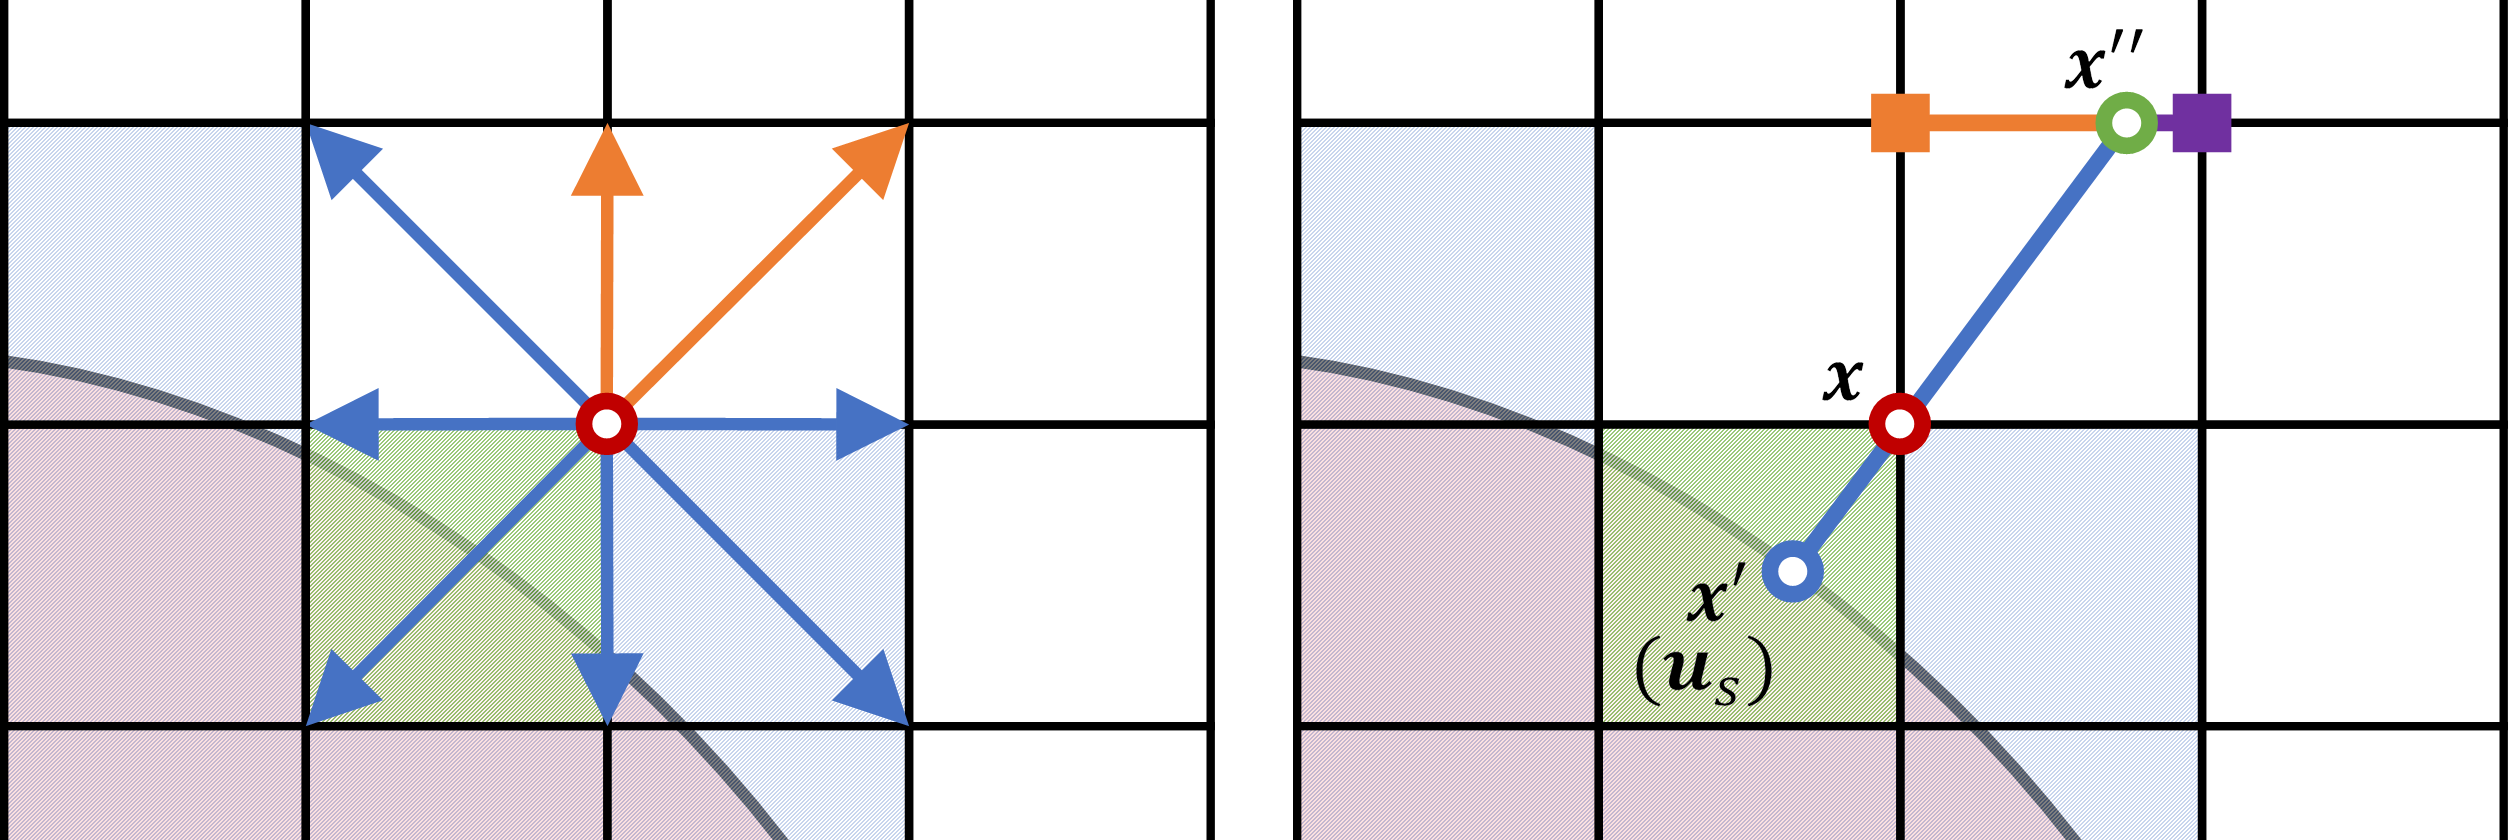
\includegraphics[width=0.95\columnwidth]{figures/cutcell_and_interpolation.png}
    \bicaption[切削网格中的速度插值]{切削网格中的速度插值。左图:因为固体边界存在而产生的切削网格 (图中标为绿色)。右图:流体中的切削网格格点$\bm{x}$ (图中标为红色圆圈) 的速度,需要通过固体边界的投影点$\bm{x}{'}$ (图中标为蓝色圆圈),与该投影点到格点的延长线与下一个网格的交点$\bm{x}{''}$ (图中标为绿色圆圈) 进行速度的线性插值得到。}{Interpolation of velocity on cut-cell nodes. Left: cut-cell (marked in green) intersecting a solid boundary; Right: the velocity on a cut-cell node $\bm{x}$ inside the fluid region (red circle) needs to be interpolated using the velocities of its projected point $\bm{x}{'}$ onto the solid boundary (blue circle) and the intersected point between the ray from the projected point to the cut-cell node and the interpolated fluid point $\bm{x}{''}$ (green circle), where the velocity can be reliably evaluated through simple linear interpolation.}
    \label{img:cutcell_and_interpolation}
\end{figure}

\begin{figure}[htb]
    \centering
      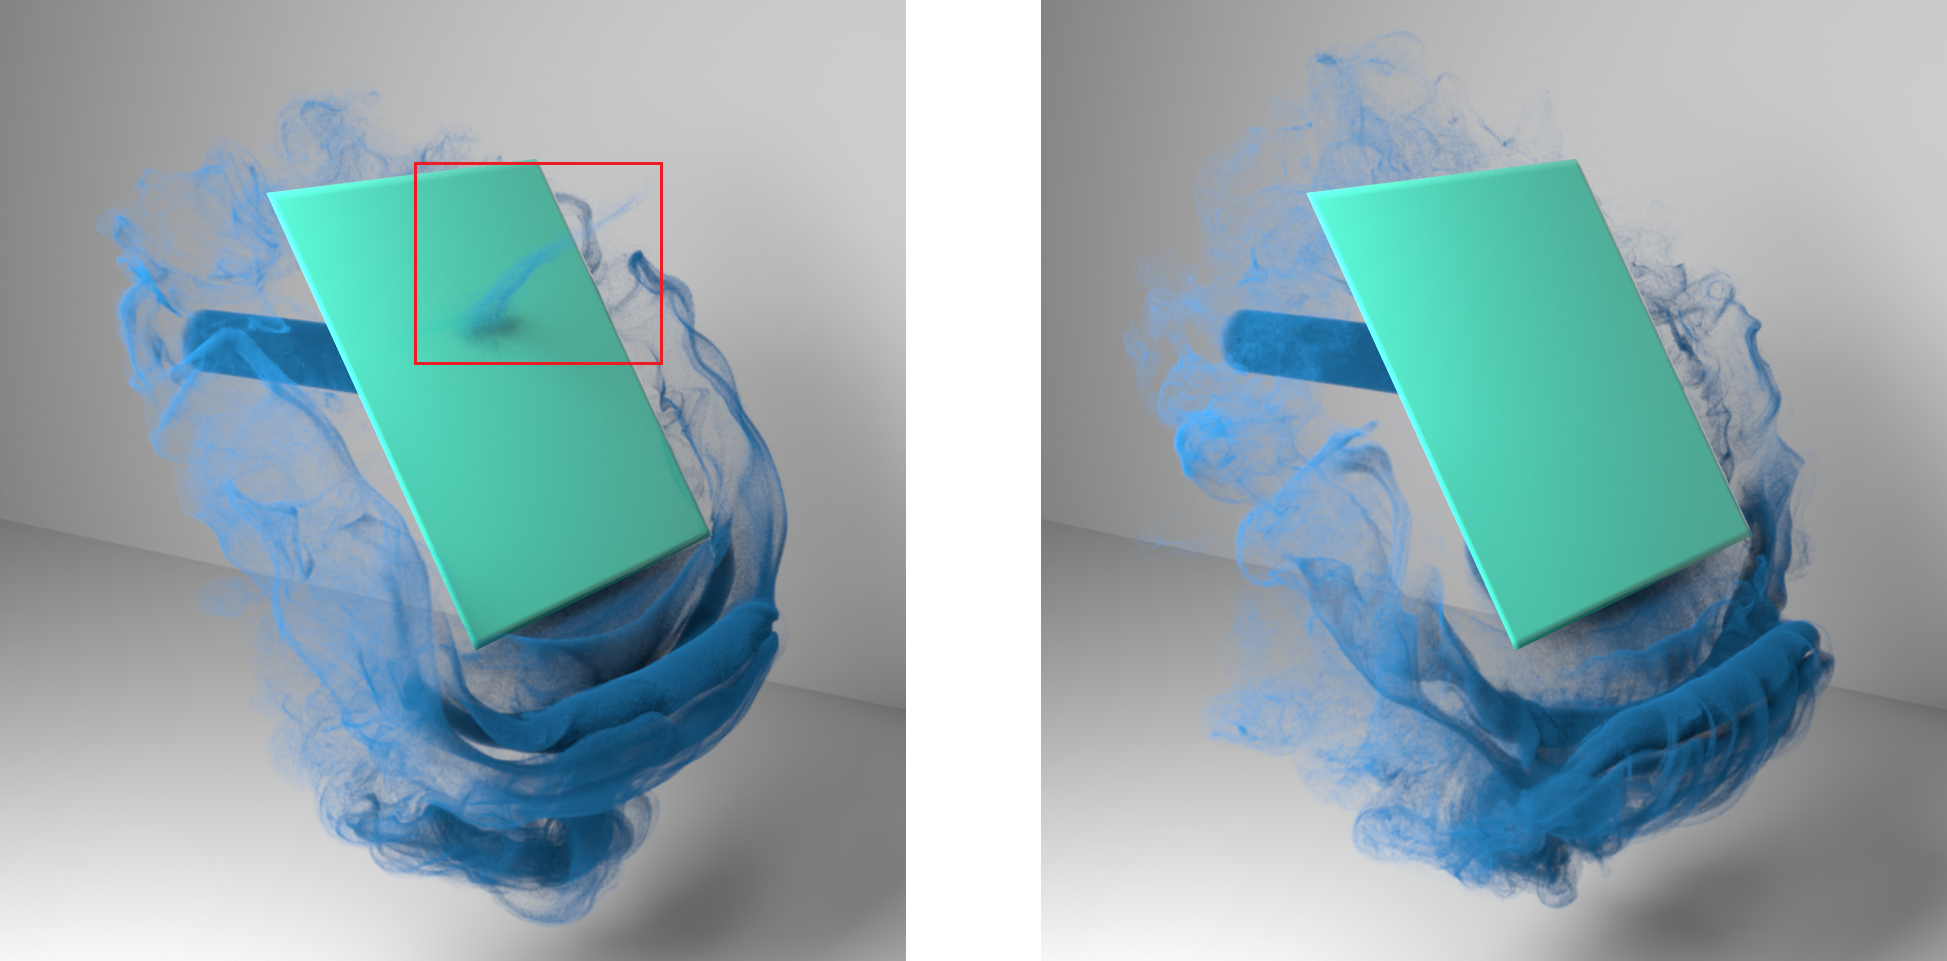
\includegraphics[width=0.97\columnwidth]{figures/comparison_with_ib.png}
    \bicaption[浸没边界法造成的泄露]{浸没边界法造成的泄露。当有薄板存在时,\citet{Li-2020} 所使用的浸没边界法 (左图) 与我们的方法的对比 (右图)。因为惩罚力会分布到薄板两侧,扩散边界浸没边界法可能会产生泄露 (见图中红色方框),而我们的方法可防止此现象。}{Leakage of immersed boundary. For a kinetic fluid simulation coupled with a thin plate, the immersed boundary method used by \citeten{Li-2020} (left) is compared with our method (right). Due to force spreading in both sides of the thin plate, this recent coupling approach employing a diffuse-interface immersed boundary method may generate leakage through the plate (see red box), while our method prevents this issue by design.}
    \label{img:comparison_with_ib}
\end{figure}

\begin{figure}[htb]
    \centering
      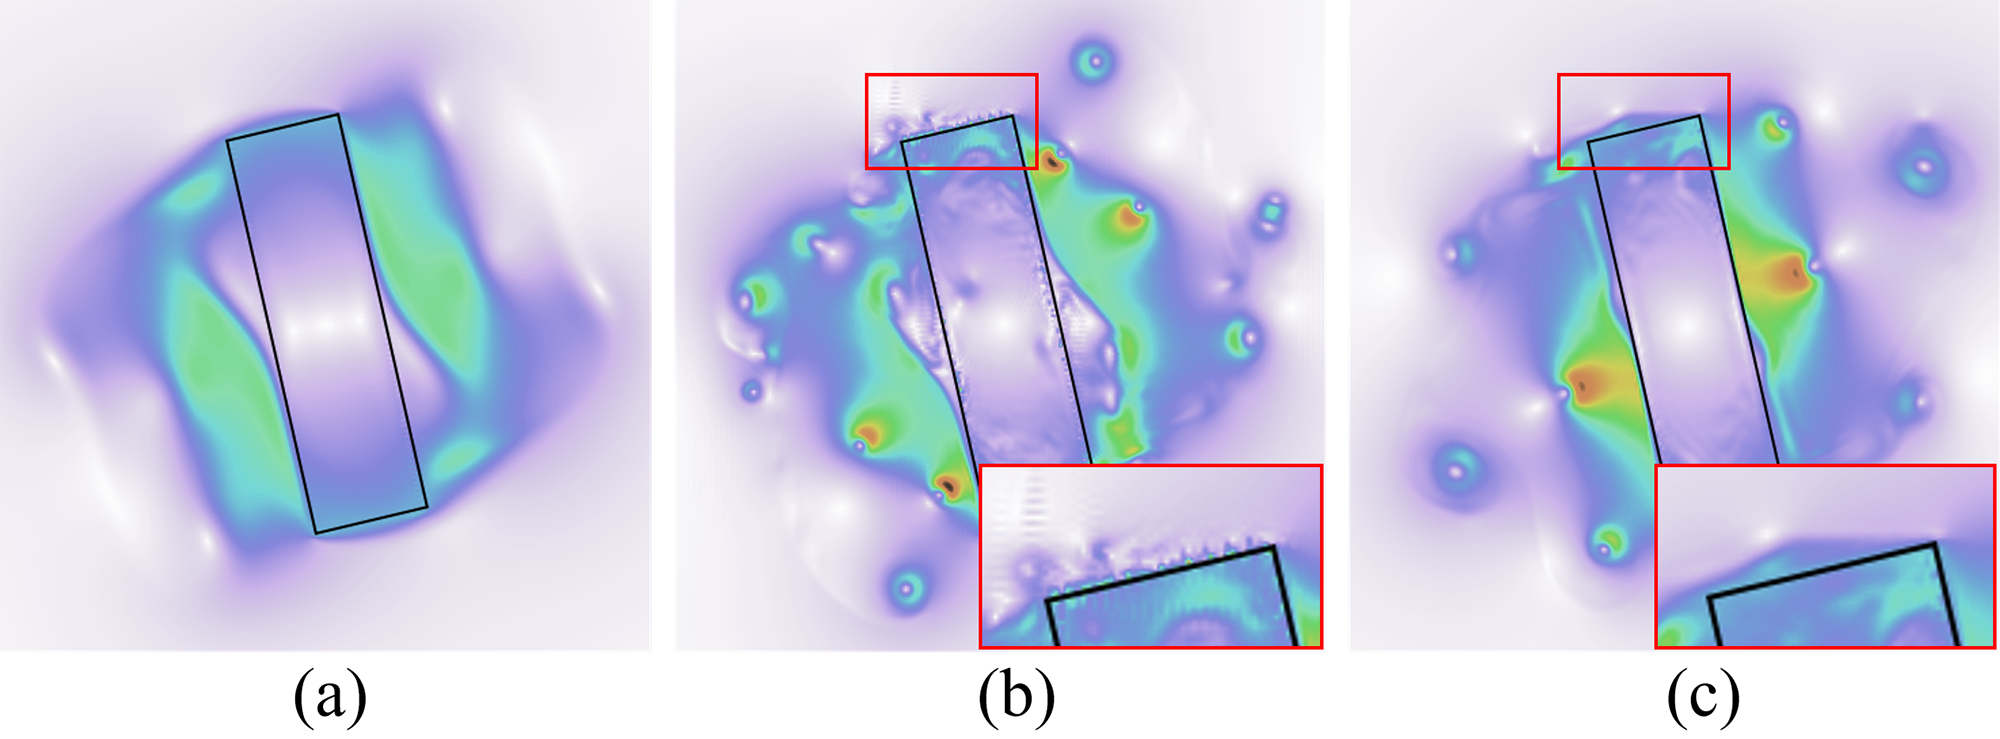
\includegraphics[width=0.95\columnwidth]{figures/ib-mbb.png}
    \bicaption[不同雷诺数下的简单反弹边界处理方法]{不同雷诺数下的简单反弹边界处理方法。(a) 在低雷诺数下,简单反弹边界没有造成视觉不正确的现象;(b) 但在高雷诺数下,固体边界会有很强的锯齿现象,从而对稳定性有较大影响;(c) 我们的方法在与 (b) 同样的高雷诺数情况下看不到视觉不正确的现象。}{Simple bounce-back under different Reynolds numbers. (a) a plain simple bounce-back scheme generates no visual artifacts for  flows with low Reynolds number; (b) however, it exhibits strong aliasing artifacts near the solid boundary for high Reynolds number flows, which may seriously influence stability; (c) our new boundary treatment for the same high Reynolds number as in (b) is artifact-free, generating the type of vortices expected from such an example.}
    \label{img:Immersed_Bounce_back}
\end{figure}

% Sec 3.2
\section{方法}
我们的混合方法主要包含下面三个部分:
\begin{itemize}
\item 双面简单反弹边界:我们首先介绍一个简单反弹边界方法的变种,即切削网格边界的两侧都会发生分布函数的反弹,而不只在一侧发生,从而不再需要追踪格子随物体运动的状态变化;
\item 切削网格的速度修正:我们通过在切削网格内进行单边的速度修正,大幅提升仿真的稳定性,同时压制边界上的速度误差;
\item 固体受力:最后我们通过介观与宏观的混合,求出流体转移至固体的动量,从而获得固体受力以驱动固体运动。
\end{itemize}

我们将在下面依次介绍这三部分内容。

\subsection{双面简单反弹边界}
在第~\ref{sec:boundary_treatment} 节中,我们回顾了简单反弹边界方法。一般来说,反弹边界都只应用于流体点。然而随着物体的运动,流体点可能被固体覆盖成为固体点,固体点也可能重新变为流体点。这个转换过程不止需要追踪格点状态,并且需要进行速度的插值,甚至外插,来完成格点的重建。这样会在高雷诺数下在固体边界上产生很强的耗散误差。为了避免这一现象,我们对所有切削网格内的点都进行分布函数反弹,而不只针对流体点。我们称该方法为双面简单反弹边界方法。这样的话,我们就不再需要区分固体点和流体点,并进行相关的格点追踪与重建。该方法依旧可以避免流体泄露,即使有亚网格物体存在。但这并没有改善固体边界的速度锯齿现象与大速度梯度造成的误差,所以我们引入下一节中介绍的速度修正方法。

\subsection{切削网格的速度修正}
我们期望获得一个速度的修正,那么势必我们需求一个理想的速度的分布,即我们认为正确的速度分布是什么样子。因为我们在这里主要考虑如何高效、灵活地处理复杂几何,而不是纯粹地追求精度,在平衡精度、效率与实现的难易度后,我们在这里谋求一个一阶 (线性) 精度的边界处理。我们注意到简单反弹边界本身也是一阶精度的,这也是我们没有采用更高阶的插值反弹边界的原因。我们在后面也通过一系列的结果展示,这一方案在实现较为简洁的前提下,对于如视觉动画制作这样的应用已经足够。我们在第~\ref{chap:sig23} 章中会介绍更高阶精度的边界处理方法,以进一步扩展我们的方法的应用范围。

当我们确立出发点为谋求线性精度的边界处理后,我们提出在双面简单反弹边界之后,通过沿固体边界的法向方向对速度线性插值,来对速度场进行修正。修正的方式为对流场施加惩罚力。更具体地说,我们先通过切削网格点周围的固体和流体速度线性插值,得到一个切削网格点上的期望速度。之后通过当前速度与期望速度的差计算惩罚力,从而修正速度场。

\paragraph{切削网格点上的期望速度}
虽然切削网格点上的期望速度是未知的待求量,但其邻近的一些点的速度是可靠的。可靠是指,这些点的速度是确定的 (如固体表面的速度) 或已知的 (如远离边界的流体点)。那么切削网格点上的期望速度可以由这些可靠速度插值得来。一个比较简单的情况是处于固体内部的切削网格点,因为它们的期望速度应与那一点的固体速度一致,而这个速度可以通过固体的运动状态直接获得。

比较复杂的情况是,处于流体中的切削网格点。对于这些点,我们需要通过一个线性插值,获得其期望速度。该插值方法如图~\ref{img:cutcell_and_interpolation} 中右图所示。对于切削网格点$\bm{x}$点,我们首先计算它在固体边界的投影点位置$\bm{x}'$,之后从$\bm{x}'$向$\bm{x}$打一条射线,该射线与下一个网格面的交点为$\bm{x}''$。如果这个面上的所有点都不是切削网格点,$\bm{x}''$点的速度就可以通过该面上的点线性插值得来 (二维中是线性插值,三维中是双线性插值)。如果这个面上存在点是切削网格点,则可寻找下一个交点,直到找到满足条件的交点。此时$\bm{x}$点的期望速度则可通过线性插值得到:
\begin{equation}  \label{eq:vel_lerp}
\hat{\bm{u}}(\bm{x})=(1-\alpha)\bm{u}_s + \alpha \bm{u}(\bm{x}'')\;,
\end{equation}
其中$\alpha=\|\bm{x}-\bm{x}'\|/\|\bm{x}''-\bm{x}'\|$,$\bm{u}_s$是固体边界上投影点$\bm{x}'$的速度。

\paragraph{基于惩罚力的速度修正}
由于切削网格点$\bm{x}$上的期望速度$\hat{\bm{u}}(\bm{x})$可能与分布函数反弹后的宏观速度$\bm{u}(\bm{x})$有偏差,我们构造如下的惩罚力$\bm{F}_p(\bm{x})$
\begin{equation} \label{eq:penaltyForce}
\bm{F}_p(\bm{x}) = \hat{\bm{u}}(\bm{x})-\bm{u}(\bm{x})
\end{equation}
施加在点$\bm{x}$上,具体的力在LBM中的实现方法与~\citep{Li-2020} 中相同,即将惩罚力投影至分布函数空间,分布函数使用最高阶的Heimite多项式展开,以维持精度与稳定性。由于反弹边界已经承担了大部分的边界处理,这里的惩罚力会比传统浸没边界法中的惩罚力小很多,只作为一个速度的修正出现,于是我们也不需要采用~\citep{Li-2020} 中的时间重缩放来缩短物理时间步长从而提升稳定性。这可以使仿真效率进一步提升。

\begin{figure}[htb]
    \centering
      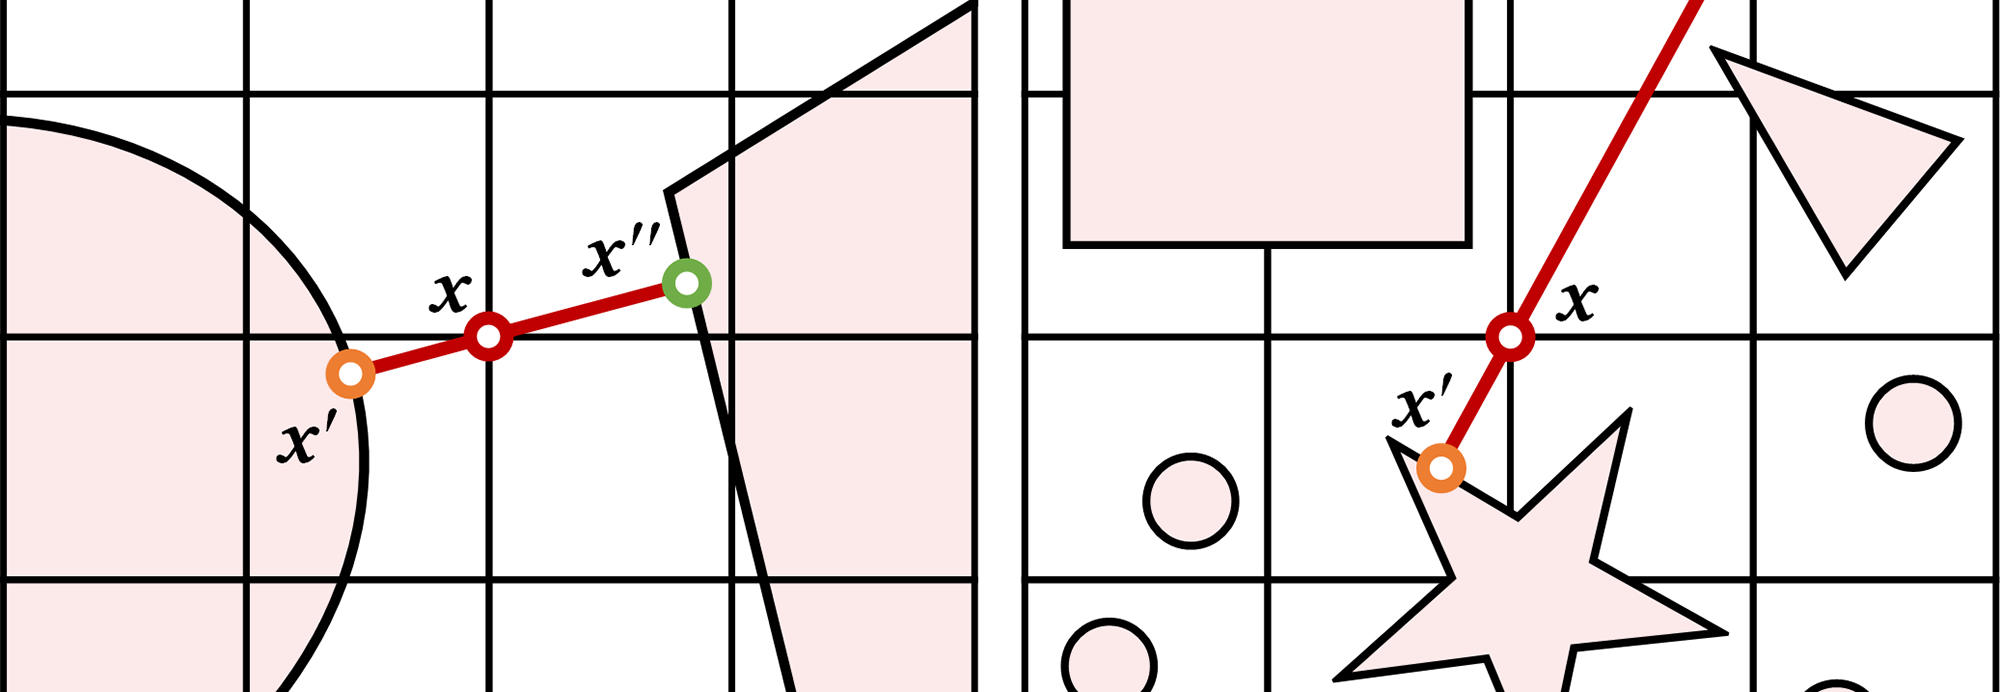
\includegraphics[width=0.95\columnwidth]{figures/cutcell_special_cases.png}
    \bicaption[两种邻近物体的情况]{两种邻近物体的情况。左图:从固体边界点$\bm{x}'$起始的射线经过$\bm{x}$点,在交到网格面之前,便相交于另一个物体上。这种情况,$\bm{x}''$是另一个固体边界点。右图:一个切削网格点可能完全被切削网格面包围,所以找不到任何非切削网格面。}{Two cases of solid proximity. Left: the ray starting from a boundary point $\bm{x}'$ through a grid node $\bm{x}$ may hit another boundary surface point before it intersects with the non-cut-cell face; in this case, $\bm{x}''$ locates at another boundary point. Right: a cut-cell node may be surrounded by all cut-cell faces, so a ray may not hit any non-cut-cell face nearby.}
    \label{img:handling_proximity}
\end{figure}

\paragraph{一些特殊情况}
当流体中的物体间距离接近网格尺度的时候,有时$\bm{x}''$的速度会无法从周围的非切削网格点插值得到。一种情况是从$\bm{x}'$点射出的射线在交到网格面之前,便相交于另一个物体上 (图~\ref{img:handling_proximity} 中左图)。那么由于这个交点的速度是已知的,我们可以用这一速度替代先前提到的非切削网格点的速度。另一种情况是,因为物体之间过于接近,射线无法找到任何非切削网格面。这个时候我们只得抛弃速度修正过程,而只采用双面简单反弹边界作为边界处理。

\begin{figure}[htb]
  \centering
    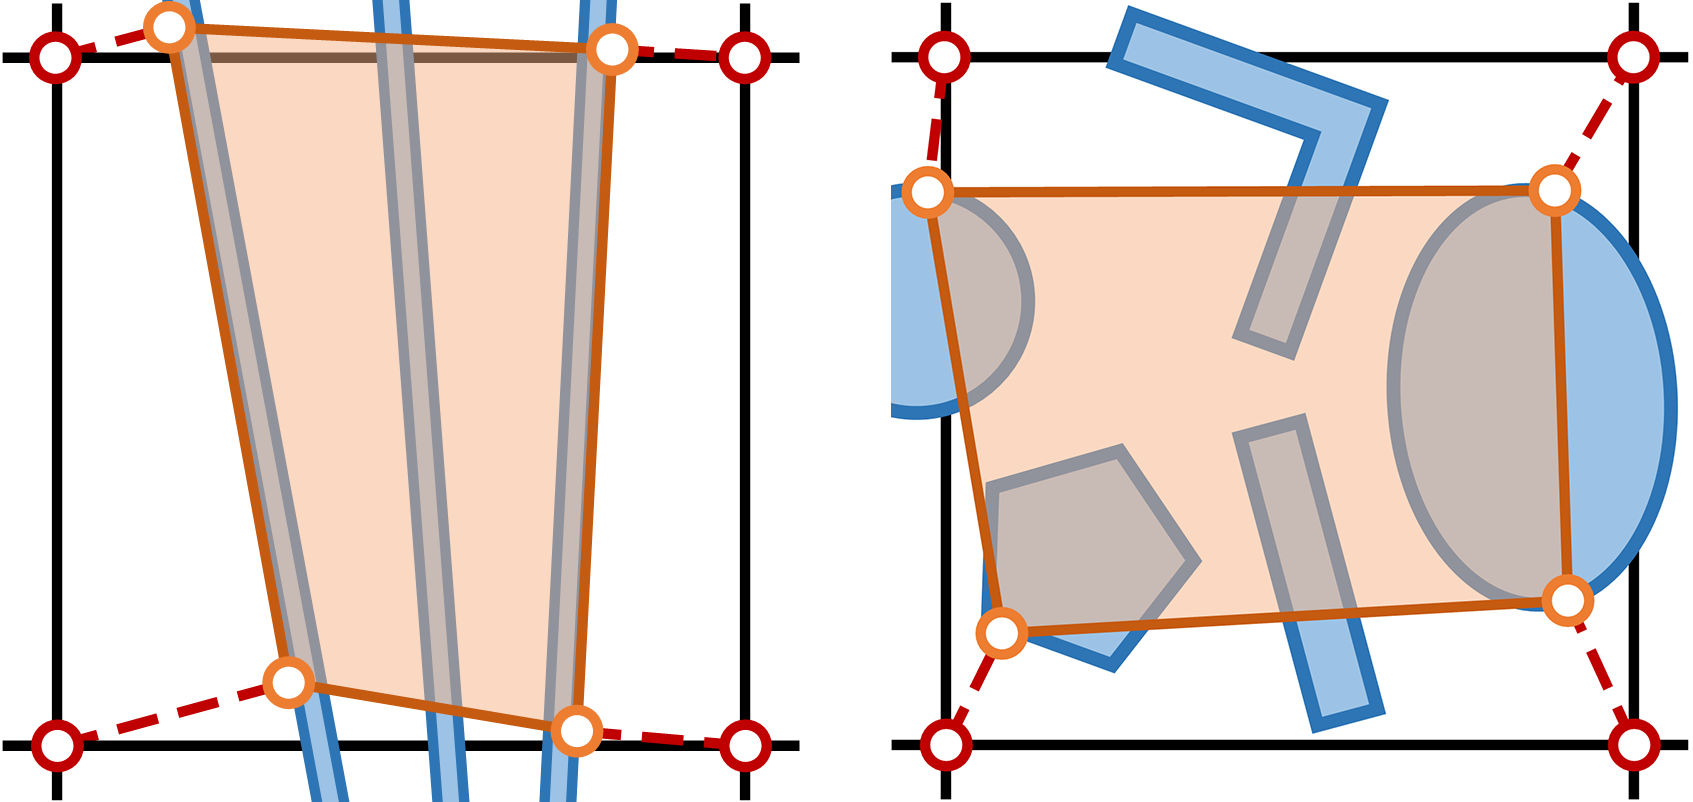
\includegraphics[width=0.9\columnwidth]{figures/sub_grid_approximation.png}
  \bicaption[亚网格近似]{亚网格近似。在亚网格物体存在时,我们将每个切削网格点投影至其最近的边界采样点。这等同于使用一个包围体积 (橘色区域) 来近似一个网格中的多个亚网格物体。}{Sub-grid approximation. To handle sub-grid scale solid structures, we project each cut-cell node onto its nearest boundary sample point. This basically amounts to using bounding volumes (orange regions) to approximate multiple thin structures within a cut-cell.}
  \label{img:sub_grid_approximation}
\end{figure}

\paragraph{亚网格近似}
当数量众多的薄板或细棒存在时,有可能一个流体网格中会包含多个这样的物体。这种情况下受制于有限的分辨率,精确地求解这些物体边界是无法做到的,尤其在网格较粗的情况中 (见图~\ref{img:sub_grid_approximation})。此时,我们使用一个包围体积,来近似这些存在于一个网格中的多个物体。所以我们依然可以将流体点投影至距离最近的固体边界点来计算惩罚力。

\paragraph{讨论}
我们的惩罚力修正是基于法向方向的线性速度插值。这个修正在比较抽象的层面可以被认为是一个滤波器,来压制在高雷诺数下,简单反弹边界造成的固体边界周围的速度震荡。这个修正可以有效地提升在湍流流固耦合仿真的稳定性,使得我们在相对粗糙的网格中也能获得视觉上可信的仿真结果。然而,这依然只是一个一阶的线性修正,所以要获得高物理精度的仿真需要高分辨率网格作为基础。但考虑到我们的动机是灵活、高效地求解复杂几何物体,我们不考虑在构造更加复杂的速度修正方法。

\subsection{固体受力}
因为要做到流固的双向耦合,我们需要讨论流体中固体的受力,也即流体传递给固体的动量。我们在边界中使用了反弹边界与速度修正的结合,所以我们在讨论固体受力时也分为两部分来讨论。我们首先讨论双面反弹边界对固体受力的贡献。在双面反弹边界之后,我们先将由公式~\ref{eq:bounce-back} 带来的动量交换进行累计。更具体地说,迁移过程后,$t$时刻$\bm{x}$点的动量可以表达为
\begin{equation}
  \bm{p}(\bm{x}) = \sum_{i \in L}\bm{c}_if^*_i(\bm{x},t).
\end{equation}
其中$L$是$\bm{x}$点切削速度方向的集合 (即与固体边界相交的速度方向)。$\bm{c}_i$方向的流固动量交换是
\begin{equation}
  \smash{\bm{c}_{i'}\,(f^*_{i}(\bm{x}) + f^*_{i'}(\bm{x}))}.
\end{equation}
从而,在$\bm{x}$点交换的动量和$\Delta \bm{p}$为
\begin{equation}
\Delta \bm{p}(\bm{x})= \sum_{i \in L} \bm{c}_{i'}\,(f^*_{i}(\bm{x}) + f^*_{i'}(\bm{x})),
\end{equation}
其中我们不将$(\Delta x)^3$显式写出 ($\Delta x$是网格大小),因为在正则化LBE空间中这一项为1。
那么反弹边界部分所贡献的固体受力是所有点动量交换的和,即
\begin{equation}
\bm{F}_{B}\equiv \sum_{\bm{x}} \Delta \bm{p}(\bm{x}),
\end{equation}
其中$\Delta t$ (时间步长) 也被隐去,因为其在正则化LBE空间中也为1。类似地,我们可以获得总的力矩
\begin{equation}
\bm{\tau}_{B}\equiv \sum_{\bm{x}} (\bm{x}-\bm{x}_{C})\times\Delta \bm{p}(\bm{x}),
\end{equation}
其中$\bm{x}_{C}$是物体质心的位置。

接下来我们继续讨论速度修正对固体受力的贡献。我们认为这个速度修正的来源依旧是固体的存在,所以这个力的来源是固体本身。那么固体理应受到一个与惩罚力大小相同,方向相反的反作用力。那么这一部分固体所受到的合力$\bm{F}_{C}$与合力矩$\bm{\tau}_{C}$可以表达为
\begin{equation}
\bm{F}_{C} = - \sum_{\bm{x}}\bm{F}_p(\bm{x}), \quad \bm{\tau}_{C} = - \sum_{\bm{x}} (\bm{x}-\bm{x}_{C})\times\bm{F}_p(\bm{x}).
\end{equation}
那么固体受到的合力$\bm{F}_s$与合力矩$\bm{\tau}_s$是上述两部分贡献的和:
\begin{align}
  \begin{split}
    \bm{F}_s = \bm{F}_{B} + \bm{F}_{C} ,\\
    \bm{\tau}_s = \bm{\tau}_{B} + \bm{\tau}_{C} .
  \end{split}
\end{align}

\section{碰撞模型的选择}
\label{sec:collision_selection}
在介绍了我们的新的边界处理方法后,我们需要选择碰撞模型。在使用本章中介绍的方法进行仿真时我们均使用第~\ref{sec:background_acmmrt} 节中介绍的自适应中心矩碰撞模型。这一选择的原因是在本文的工作提出前,自适应中心矩碰撞模型是图形学中最先进的碰撞方法。这使得我们可以排除碰撞模型的影响,与图形学中的现有方法进行对比。并且我们展示该碰撞模型的能力对图形学中的应用是足够的。我们注意到累积量碰撞模型 (第~\ref{sec:cumulant} 节) 的一些理论优势,但同时也注意到由于其发展时间较短 (最早的工作见于~\citep{Geier-2015}),发展还并不完善。我们会在第~\ref{chap:sig23} 章中对现有累积量模型的改进与应用进行详细讨论。

\section{算法优化}
\subsection{几何近似}
我们的混合边界处理中需要许多的几何计算,如将流体点投影至固体表面,或将速度方向与固体边界进行求交等。我们还需要识别切削网格点,以及它们的状态 (属于流体区域或固体区域)。许多工作阐述了如何准确地进行这样的几何计算~\citep{Azevedo-2016,Robinson:2009}。但由于固体边界的形状可能十分复杂,这一过程可能非常耗时,不利于维持LBM高并行度的优势。
为了在效率与精度间取得平衡,我们提出一系列的几何近似计算方法,以在不影响视觉可信度的情况下提升计算效率。

\begin{figure}[!htbp]
  \centering
    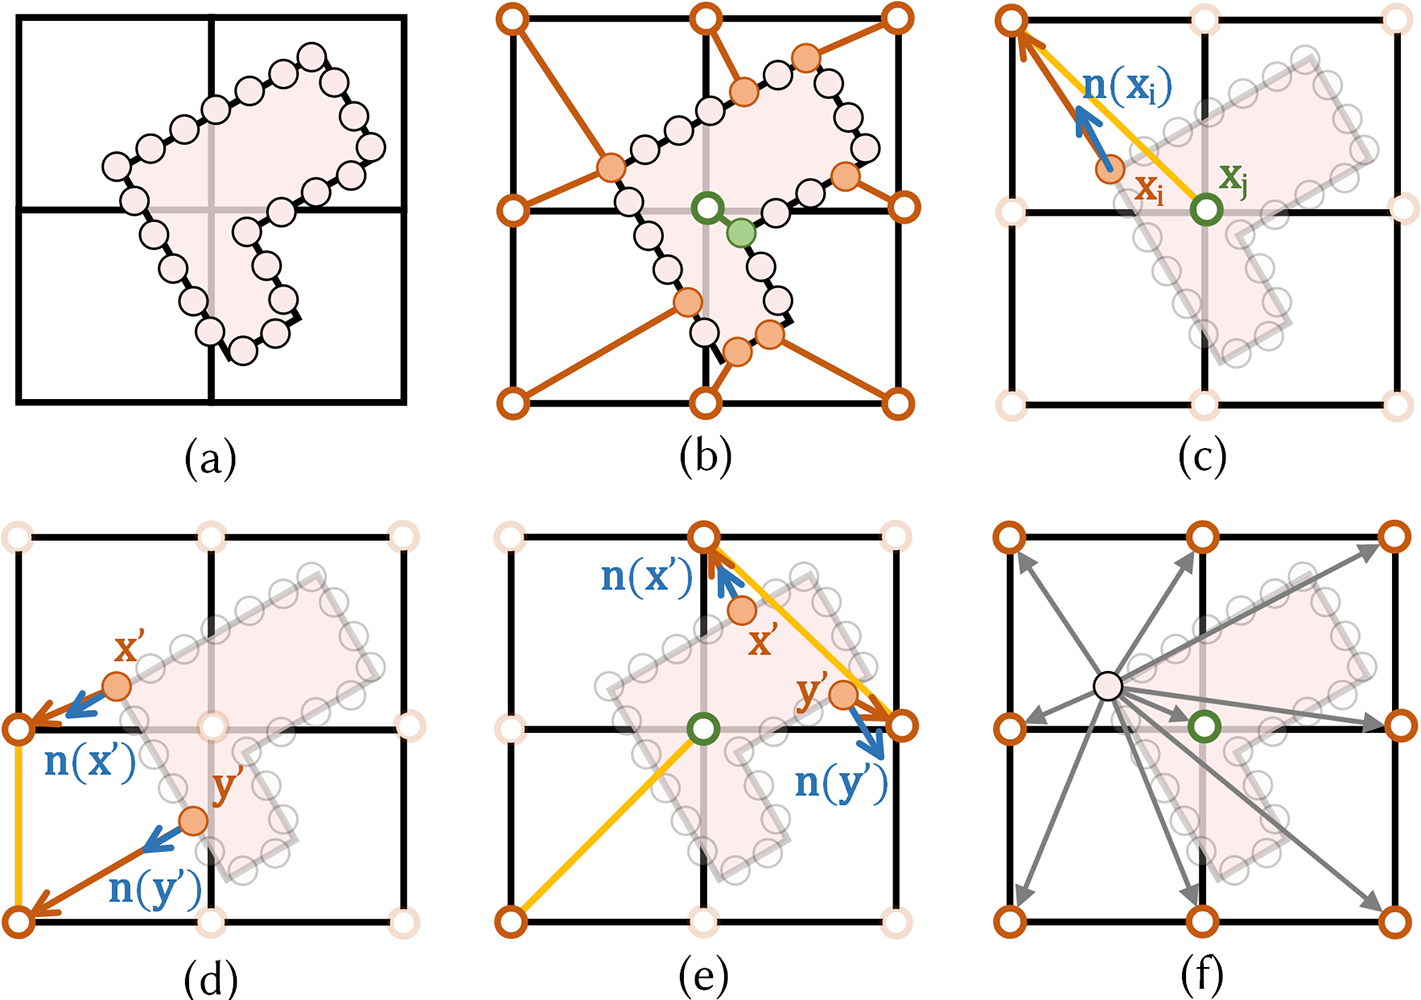
\includegraphics[width=0.92\columnwidth]{figures/geometric_computing.png}
  \bicaption[高效几何近似计算]{高效几何近似计算。对于一个固体,我们首先对它的边界采样 (a),然后切削网格点的投影点可以被近似为距其最近的采样点 (b)。为了检验某个速度方向 (图中标为黄色) 是否与固体边界相交,我们可以检查这个方向的两端是否有固体点存在。如果一端是固体点另一端是流体点,则我们认为其跨过了固体边界 (c) (图中绿色点为固体点,橘色点为流体点)。对于两端都是流体点的情况,我们检查这两个流体点投影点的法向,如果它们有类似的朝向 (d) 则认为该方向没有跨过边界,相反则认为其跨过边界 (e)。在GPU实现时,我们从所有的固体采样点出发,令每个固体采样点寻找其周围的流体切削网格点,而不是从流体点出发。}{Efficient geometric approximation. Given a solid geometry, we first sample its boundary (a); then the projected points of cut-cell nodes can be simply approximated by the nearest sample (b). To examine whether a link (yellow) crosses the solid boundary, we first check if solid nodes are involved. If the ends of the link are fluid and solid nodes, then it crosses the solid boundary (c) (green cut-cell nodes are inside the solid, whereas orange ones are in the fluid). For links connecting fluid nodes, we check the normals of the two projected cut-cell nodes forming the link; if the two normals have the same orientation (d), the link does not cross the solid boundary; otherwise, it intersects the solid boundary (e). For GPU implementation, we parallelize over solid samples instead of cut-cell nodes, where each solid sample will check its surrounding region of cut-cell nodes.}
  \label{img:geometric-computing}
\end{figure}

\paragraph{表面采样与切削网格识别}
为了加速计算,我们可以使用采样点而不是实际的几何来表达边界。这一过程需要对固体表面进行均匀采样,如使用泊松圆盘采样 (Poisson-disk sampling)~\citep{dunbar2006spatial}。注意这也要求固体模型应该是密封的。每一个采样点$\bm{x}_s$在采样时可获得一个由边界朝外的法向$\bm{n}(\bm{x}_s)$。之后如果有网格中包含至少一个边界采样点,这个网格就可以被识别为切削网格 (如图~\ref{img:geometric-computing} (a))。

\paragraph{高效切削网格投影}
在几何计算中一个最重要的 (也可能是最耗时的) 部分是将流体点$\bm{x}$投影至固体表面上,以得到投影点位置$\bm{x}'$。传统方法可能会构建一个树形结构,然后搜索距离$\bm{x}$点最近的三角形~\citep{wang-2012}。在这里我们使用一个高效的近似算法来替代这一过程,我们在固体表面选择一个距离$\bm{x}$点最近的采样点$\bm{x}_s$,并满足
\begin{equation}\label{eq:is_in_fluid}
(\bm{x}-\bm{x}_s)\cdot \bm{n}(\bm{x}_s) \geq 0\;
\end{equation}
来近似采样点$\bm{x}'$。公式~\ref{eq:is_in_fluid} 这个约束可以避免我们选择到错误朝向的采样点。如果没有满足这个约束的采样点,那么这个点应该被标记为固体点 (如图~\ref{img:geometric-computing} (b))。这个基于采样点的技术可以达到很高的并行度,但精度很显然依赖于采样密度。所以在实现中,我们需要保证每个切削网格内有足够的采样点数。一般我们设置泊松圆盘采样的采样距离不超过网格大小 ($\Delta x$) 的一半。

\paragraph{近似反弹边界处理}
在双面反弹边界处理中,我们必须要识别出与固体边界相交的速度方向 (见图~\ref{img:bounce_back_scheme})。对于厚物体,由于我们已经对切削网格点属于流体点或固体点有所标记,我们只许对速度方向的两端点的状态进行识别。如果两个端点分别为流体点和固体点,则这个速度方向与固体边界有相交。但是对于薄物体,可能存在两端均是流体点,但依然与固体表面相交的情况。所以我们要进行特殊识别。
对于从$\bm{x}$至$\bm{y}$点的速度方向,我们检查这两个点的投影点$\bm{x}'$与$\bm{y}'$的法向朝向是否不一致,即$\bm{n}(\bm{x}')\!\cdot\!\bm{n}(\bm{y'})\!<\!0$ (如图~\ref{img:geometric-computing} (d)与(e))。
如果朝向不一致 (图~\ref{img:geometric-computing} (e) 即为此情况),则我们认为$\bm{x}$点与$\bm{y}$点处于边界的不同侧,所以这个速度方向是与固体表面相交的。则我们应在这个方向上进行反弹边界处理。

\subsection{GPU实现}
目前为止所描述的我们的算法,包括几何近似,我们都希望它们尽可能的简单,且只涉及局部计算。这样可以令GPU的实现较为简单直接,且有尽可能高的计算效率。在实现时我们应用了 \citet{Chen-2021} 中提出的加速技术,与一些针对我们算法设计的加速实现。这些实现方法在本节进行讨论。

\paragraph{快速碰撞计算}
\citet{Chen-2021} 讨论了在碰撞过程中所需要的中心矩投影矩阵$\bm{M}(\bm{u})$的逆矩阵$\bm{M}(\bm{u})^{-1}$计算问题。作者们在其中提到逆矩阵应该使用解析式进行计算来保证碰撞的精度。然而由于解析式非常复杂,在GPU计算时,会占用过多的寄存器,导致GPU占用率低。但是我们注意到,如果将$\bm{M}(\bm{u})^{-1}$的解析式进行LU分解~\citep{fei2018three},分解后的三角矩阵中很多元素是非常接近于0的。所以我们可以将这些非常接近于0的元素置0,之后使用稀疏矩阵的数据格式进行存储。这样并不会影响整体计算的精度 (所造成的误差低于机器误差),但是寄存器使用量可以大幅减少。在同样的GPU上进行测试,我们的碰撞过程的效率约是~\citep{Chen-2021} 中碰撞过程的三倍。

\paragraph{存储布局}
对于LBM来说,在并行时一般是按方向的。即先计算$f_0$,之后计算$f_1$、$f_2$、……,以此类推。在这种情况下数组结构体 (structure-of-arrays, SoA) 是对缓存更友好的存储布局,因为SoA结构可以提升缓存利用率,从而提升整体性能~\citep{Chen-2021}。我们在实现中也同样使用SoA布局。

\paragraph{并行的切削网格点识别与投影}
我们在上一小节讨论了我们算法中的一个关键步骤是将切削网格点投影到物体表面,这一过程可以通过寻找距离该点最近的固体采样点来近似。一般这一过程会将流体边界点作为并行单元,来搜索距其最近的采样点。但是这样会造成GPU负载不均衡,从而降低GPU占用率。
所以我们在这一过程中,将固体采样点作为并行单元。对于每一个采样点,我们计算该点到周围的切削网格点的距离 (见图~\ref{img:geometric-computing} (f)),并且比较这个距离与切削网格点当前记录的最近点的距离。如果距离更小的话则更新该采样点为最近点。因为多个线程可能会同时访问同一个流体点,这一过程需要使用原子比较计算。注意公式~\ref{eq:is_in_fluid} 依然需要满足,所以切削网格点状态可以被同时识别。
这样的好处是,每个固体采样点附近一定存在切削网格点,并且数量接近。这样可以大幅提升GPU的负载均衡,减少无用的线程造成的线程开销,提升GPU占用率。

\begin{figure}[!tb]
  \centering
    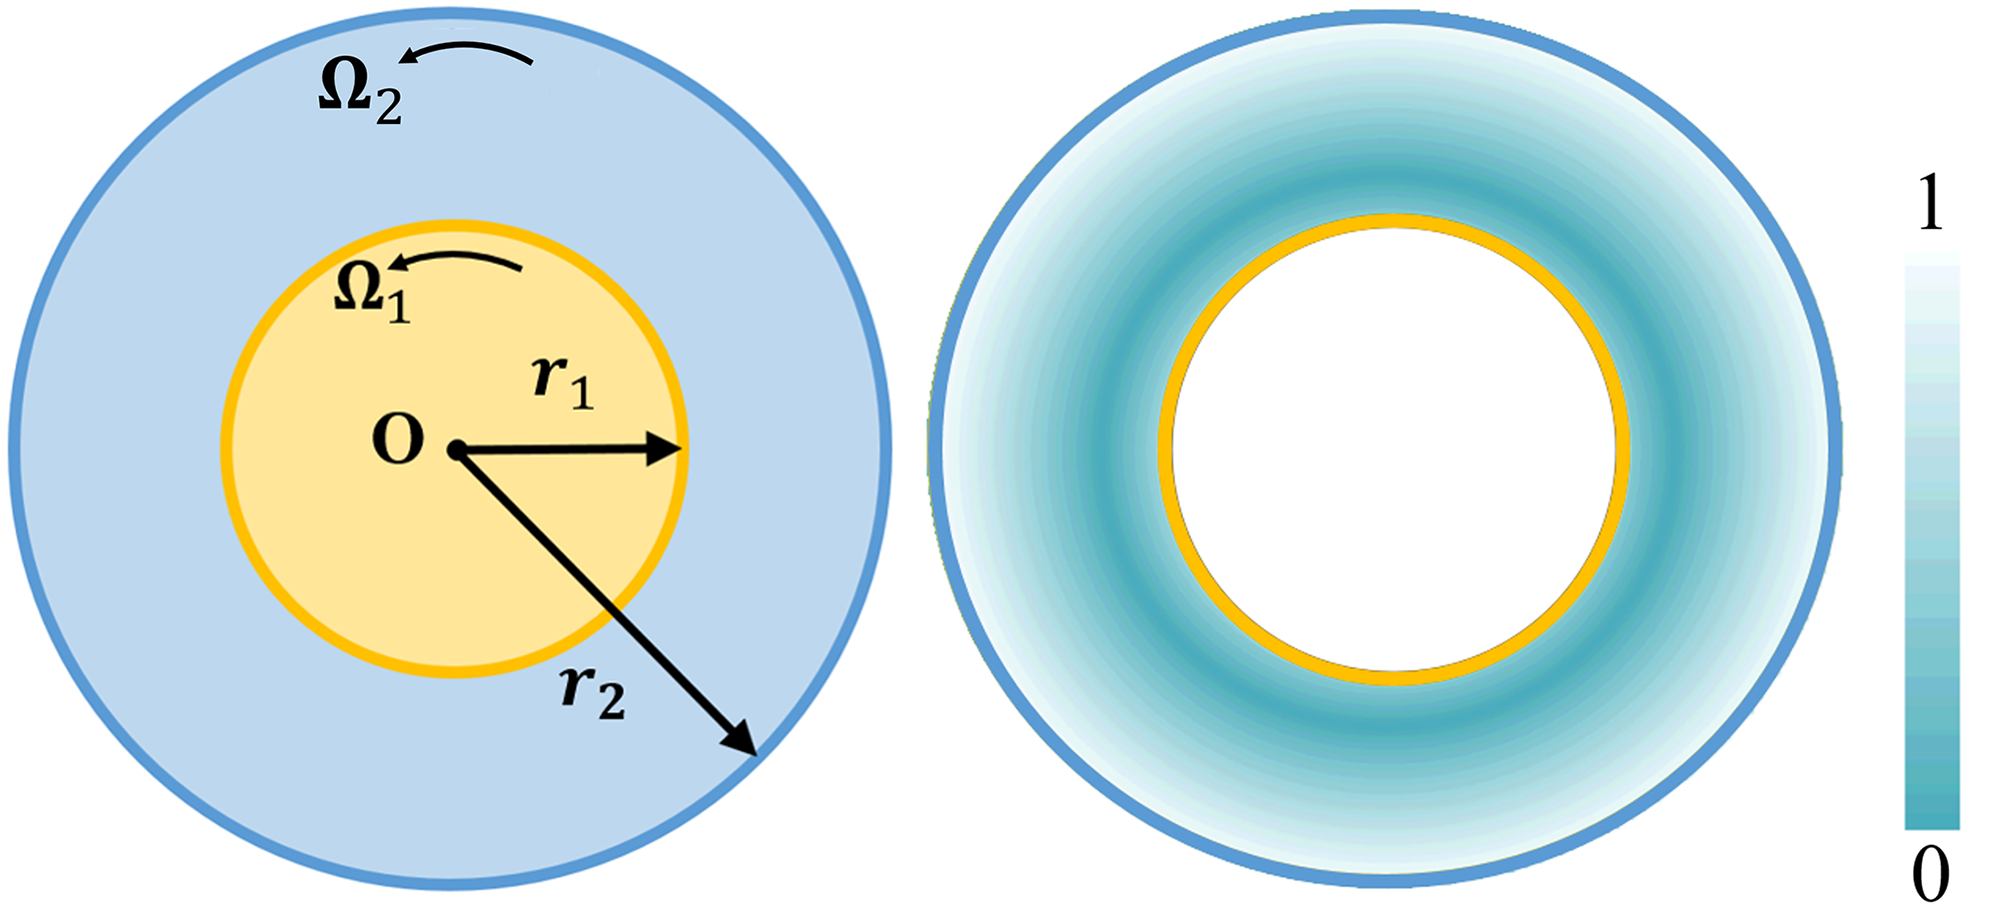
\includegraphics[width=0.8\columnwidth]{figures/taylor-couette-setting-2d.png}
  \bicaption[二维泰勒-库埃特流]{二维泰勒-库埃特流。左图:两个以$\bm{O}$点为圆心的同心圆,半径分别为$r_1$、$r_2$,角速度为$\Omega_1$、$\Omega_2$,通过旋转在中间的圆环中形成泰勒-库埃特流。右图:二维泰勒-库埃特流的解析解速度场模值的可视化。}{2D Taylor-Couette flow. Left: the Taylor-Couette flow runs between two concentric circle boundaries locating at origin $\bm{O}$ with radii $r_1$ and $r_2$ whose rotating speeds are $\Omega_1$ and $\Omega_2$, respectively. Right: visualization of velocity magnitudes of the analytical solution between two rotating circles.}
  \label{img:taylor-couette-setting-2d}
\end{figure}

\section{与现有方法的对比}
\label{sec:siga21_comp}
此节中我们将我们的图形方法与图形学中近期提出的 (也是目前最前沿的) LBM仿真方法~\citep{Li-2020} 进行定量与定性的对比。我们还针对计算效率,讨论基于 \citet{Li-2020} 所提方法的性能改进~\citep{Chen-2021} 与我们方法的比较。

\begin{figure}[!tb]
  \centering
    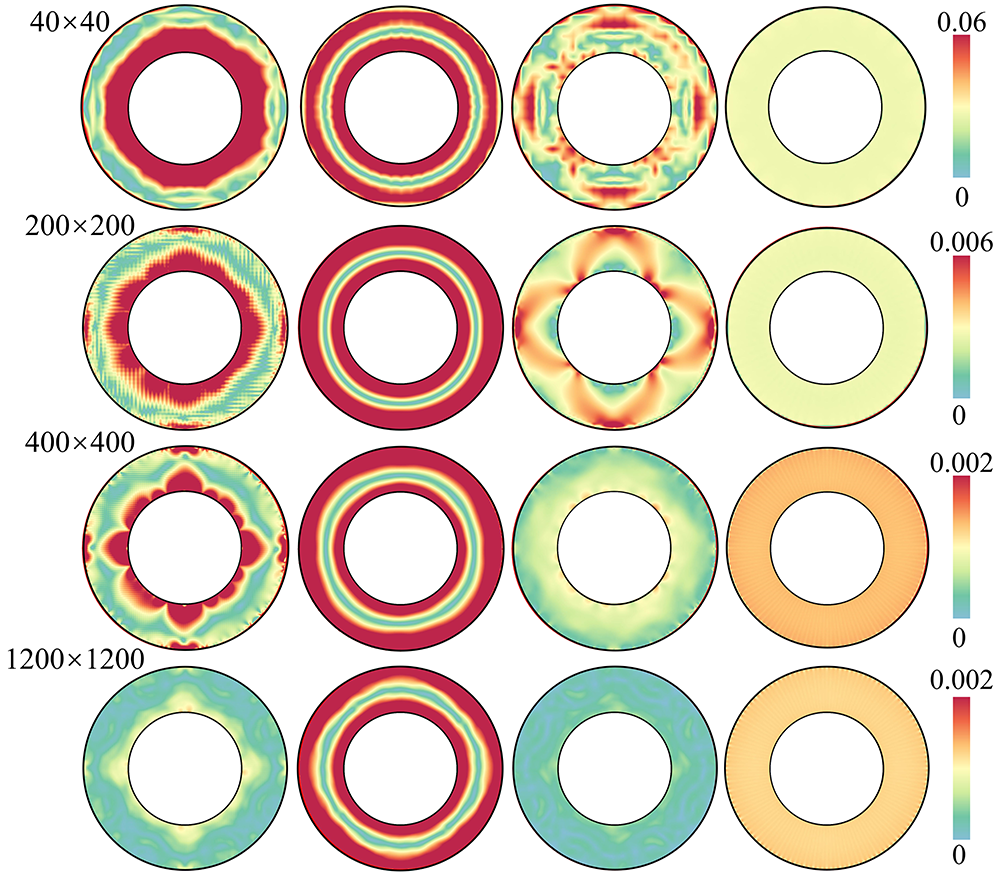
\includegraphics[width=0.94\columnwidth]{figures/taylor-couette-compare-2d.png}
  \bicaption[二维泰勒-库埃特流仿真的对比]{二维泰勒-库埃特流仿真的对比。我们将不同求解器 (从左至右) 得到的不同分辨率 (从上至下) 的二维泰勒-库埃特流数值仿真结果进行可视化,可视化的值为相对误差,场景设置见图~\ref{img:taylor-couette-setting-2d}。图中从左至右依次为原始的简单反弹边界~\citep{Ladd-1994}、\citep{Li-2020} 中的动理学方法、我们的边界处理,以及ANSYS Fluent求解器。ANSYS Fluent在求解时使用了自适应的体网格,平均元素大小与其它求解器中的网格大小相当。}{Comparison of 2D Taylor-Couette flow simulation. We visualize the relative errors of the numerical solution to the 2D Taylor-Couette flow of Fig.~\ref{img:taylor-couette-setting-2d} computed by different solvers (columns) and different resolutions (rows). From left to right: the original bounce-back scheme~\citepen{Ladd-1994}, the kinetic solver of~\citepen{Li-2020}, our boundary treatment method, as well as the ANSYS Fluent solver using adaptive radial mesh for which the average element area matches the grid cell area used for the other solvers.}
  \label{img:taylor-couette-compare-2d}
\end{figure}

\begin{figure}[!tb]
  \centering
    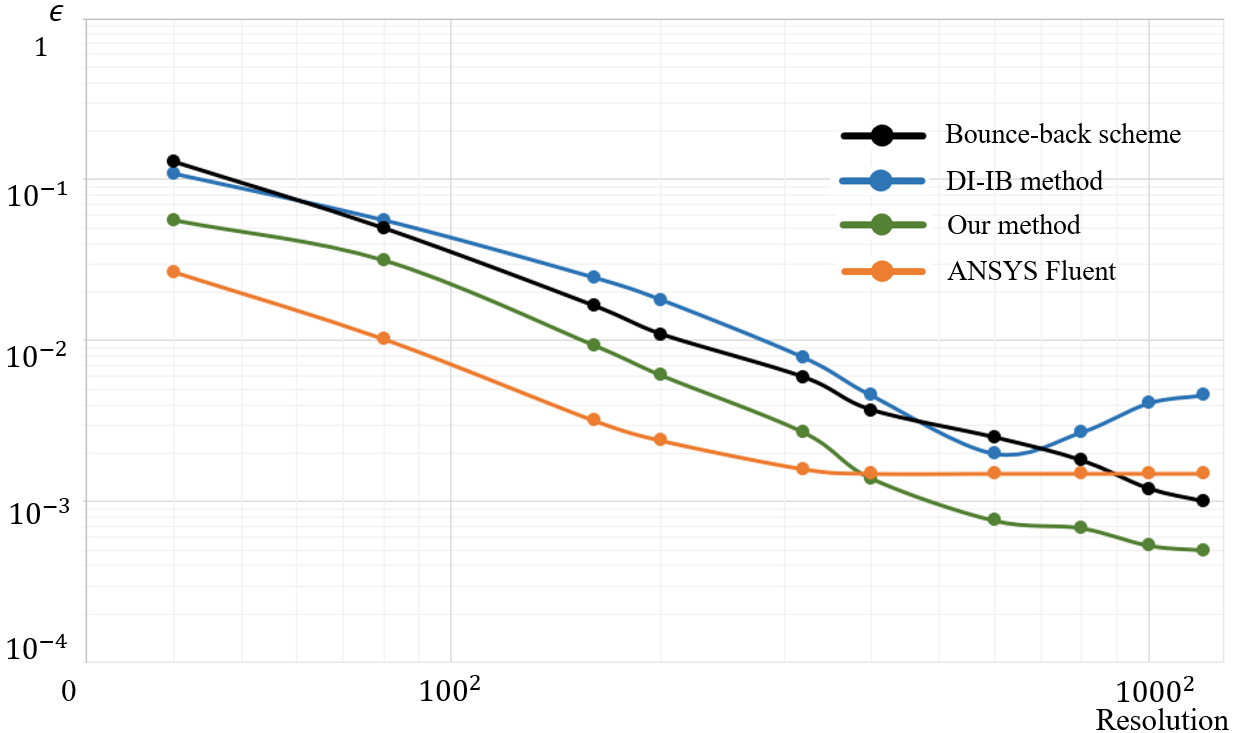
\includegraphics[width=0.94\columnwidth]{figures/taylor-couette-error-compare.png}
  \bicaption[不同类型求解器的误差收敛情况]{不同类型求解器的误差收敛情况。我们对二维泰勒-库埃特流进行仿真,并衡量了在不同分辨率下,不同类型的求解器的相对误差,以展示各个求解器的误差收敛情况。相对误差根据公式~\ref{eq:error_metric} 计算得到。}{Convergence for different types of solvers. We simulated the 2D Taylor-Couette flows with different types of solvers and measured the relative errors according to Eq.~\ref{eq:error_metric} to show the convergence for different solvers as resolution increases.}
  \label{img:taylor-couette-error-compare}
\end{figure}

\paragraph{二维泰勒-库埃特 (Taylor-Couette) 流仿真}
为了验证我们方法的精度,我们首先对二维泰勒-库埃特流进行仿真。这是一个经典的二维流体基准测试,具体来说,测试的场景为两个同心圆 (厚度可不计) 分别以各自的速度旋转~\citep{xu2006immersed}。即在这个场景中,这两个圆既为薄物体,又为动态边界,所以十分适合对我们的方法进行精度的测试。该测试场景的示意可见图~\ref{img:taylor-couette-setting-2d} (a)。
两个圆的半径分别为$r_1 \!=\! 0.5$、$r_2 \!=\! 1.0$,角速度为$\Omega_1 \!=\! 1.0$、$\Omega_2 \!=\! -1.0$。雷诺数为$\text{Re} \!=\! 10$,对应运动黏度为$\nu \!=\! 0.1$。
在这样的设置下,两个圆之间的圆环会产生流场,并且这个流场存在解析解$\bm{u}^\text{ref}\!=\!(u_x^\text{ref},u_y^\text{ref})$。我们以两个圆的圆心为坐标轴原点,对于任意一个点$(x,y)$,我们可以用$r\!=\!\sqrt{x^2+y^2}$衡量该点到圆心的距离。那么对于$r\!\in\![r_1, r_2]$的点,流场的解析解为
\begin{equation}
u_x^\text{ref} = -\bigl(A + \frac{B}{r^2}\bigr)y, \hspace{4mm} u_y^\text{ref} = \bigl(A + \frac{B}{r^2}\bigr)x\;,
\end{equation}
\noindent 其中常数$A$与$B$的定义为:
\begin{equation}
A = \frac{\Omega_2 r_2^2 - \Omega_1 r_1^2}{r_2^2 - r_1^2}, \hspace{4mm} B= \frac{(\Omega_1 - \Omega_2)r_1^2r_2^2}{r_2^2 - r_1^2}.
\end{equation}
图~\ref{img:taylor-couette-setting-2d} (b) 展示了这个解析解速度分布的可视化。

\begin{figure}[!tb]
  \centering
    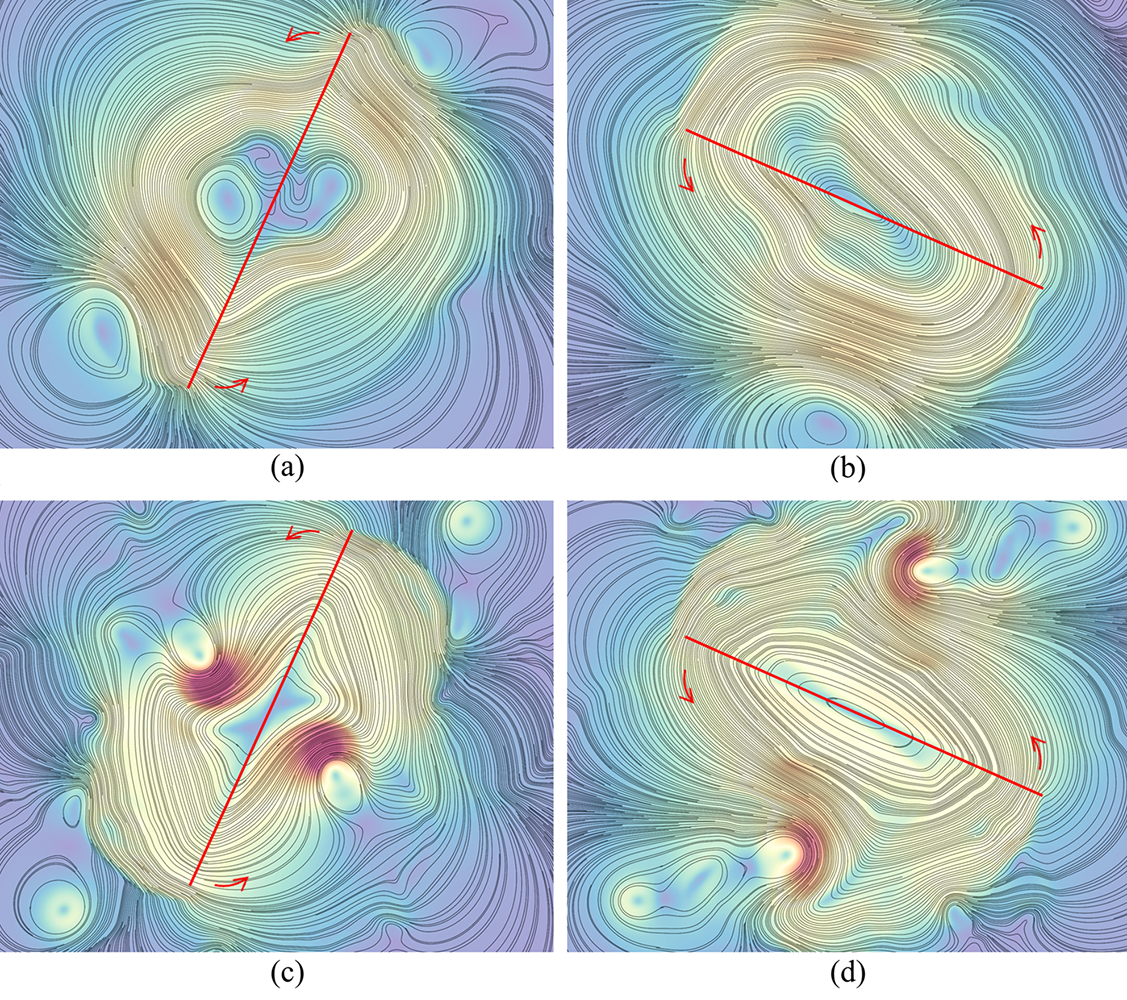
\includegraphics[width=0.99\columnwidth]{figures/ns-compare-2d.png}
  \bicaption[与二维N-S求解器的对比]{与二维N-S求解器的对比。我们仿真一个二维的薄板在流体中旋转的场景,仿真分辨率为$256\times256$。顶图:由基于切削网格方法的N-S求解器~\citep{Azevedo-2016} 得到的速度场模值;底图:我们的图形方法获得的速度场模值。(a)、(c) 与 (b)、(d) 分别从仿真中的同一帧截取。虽然两个仿真方法的结果都在视觉上可以接受,但是我们的方法有着更多涡流的细节,证明了我们的方法更适合于湍流的仿真场景。}{Comparison with 2D N-S solver. We simulated a 2D thin plate spinning in a fluid using a grid resolution of $256\times256$. Top: velocity magnitude plot from a cut-cell-based NS solver~\citepen{Azevedo-2016}; Bottom: velocity magnitude plot from our solver for the same frames as (a) and (b). Although both solvers retain good boundary velocities, ours produces much more detailed vortices, making it significantly more suitable for solving coupling in a turbulent flow scenario.}
  \label{img:cut-cell-based-NS-solver}
\end{figure}

我们使用了不同的求解器,对该边界驱动的流体进行求解,求解器分别为 (a) 使用原始简单反弹边界~\citep{Ladd-1994} 的动理学方法、(b) DI-IBM~\citep{Li-2020}、(c) 我们的图形方法与 (d) 使用N-S方法的商业求解器ANSYS Fluent~\citep{Ansys-2014}。在使用ANSYS Fluent求解时,我们采用了自适应的体网格,平均元素大小与其它求解器中的网格大小相当。由于其使用的是贴体网格,ANSYS Fluent的误差应该会更小。
图~\ref{img:taylor-couette-compare-2d} 展示了不同求解器 (从左至右) 在不同分辨率 (从上至下) 下的相对误差的分布。从图中可以看到我们的方法相比其它方法拥有更小误差同时,也随着分辨率上升而更快地达到收敛。

我们还测量了不同求解器结果的加权$\ell_2$误差:
\begin{equation}\label{eq:error_metric}
\epsilon = \frac{\sum_i w(\bm{x}_i)\|\bm{u}(\bm{x}_i)-\bm{u}^{\text{ref}}(\bm{x}_i)\|_2}{\sum_i w(\bm{x}_i)\|\bm{u}^{\text{ref}}(\bm{x}_i)\|_2}\;,
\end{equation}
其中$\bm{x}_i$是流体域中的一个格点,$\bm{u}^{\text{ref}}$是解析解,权重$w(\bm{x}_i) \!=\! 4|r-\bar{r}|$,$\bar{r}\!=\!(r_1+r_2)/2$。这个权重存在的目的是更多地体现边界附近的误差,因为我们本质上在对比边界处理。图~\ref{img:taylor-couette-error-compare} 展示了不同求解器的误差随分辨率上升的变化情况。显然,我们的图形方法比起其它两个动理学边界处理方法都有着更好的表现。并且,我们的图形方法在分辨率足够高时,也优于ANSYS Fluent。

\begin{figure}[htbp]
  \centering
    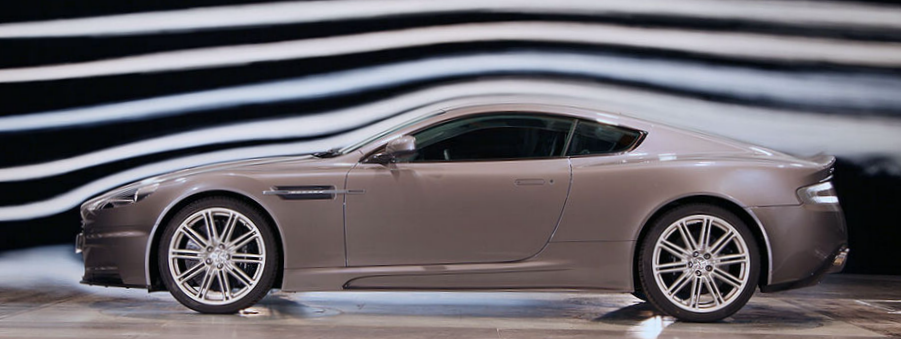
\includegraphics[width=0.99\columnwidth]{figures/car_wind_tunnel.png}
  \bicaption[汽车的风洞测试]{汽车的风洞测试。汽车周围的气流可视化展示了车身的设计使得气流直到后备箱才发生边界层分离,这样可以有效减少风阻与震动。图片版权来自\textit{Auto Motor und Sport}, \copyright Frank Herzog/Sportauto.}{Wind-tunnel test of a car. A wind tunnel visualization of the airflow around a car shows that the design of the body delays boundary layer separation until the trunk, which reduces drag and vibration in practice. Image courtesy of \textit{Auto Motor und Sport}, \copyright Frank Herzog/Sportauto.}
  \label{img:car_wind_tunnel}
\end{figure}

\paragraph{与基于切削网格的二维N-S求解器的对比}
CG领域中的N-S方法已经发展得较为成熟,且拥有一系列不同的流固耦合方法。其中基于切削网格的方法是精度与计算效率均相对较高的方法。于是我们与~\citep{Azevedo-2016} 中的基于切削网格的N-S方法进行对比。该方法在切削网格构造了类似有限体积法中的网格以提升精度。我们使用该方法与我们的图形方法分别仿真了一个二维的薄板以角速度$\omega_s = 3 \text{ } rad/s$旋转的场景,并将得到的速度场展示在图~\ref{img:cut-cell-based-NS-solver} 中。由于~\citet{Azevedo-2016} 求解的是无黏度的欧拉方程,我们在我们的仿真中也将黏度设为0 ($\nu\!=\!0$)。虽然~\citet{Azevedo-2016} 的方法得到了不错的结果,但是在流场中只有大涡,即使流体本身是无粘的,而我们的方法可以提供更多的湍流细节。我们注意到目前也有一些更加精准的N-S求解器,如~\citep{Zehnder-2018,Qu-2019},但这些方法的计算效率是显著不如动理学方法的~\citep{Li-2020}。从上述分析可得,我们的方法拥有较为独特的优势,即提供更为精准且高效的湍流仿真,同时可以对不同类型的复杂几何进行耦合。

\paragraph{与图形学中现有方法的对比}
近来,\citet{Li-2020} 提出了一个基于动理学方法的双向流固耦合湍流求解方法,该方法使用DI-IBM处理固体边界。然而这一方法有一定的局限性。首先因为DI-IBM在边界两侧施加惩罚力,其在求解亚网格物体的流固耦合时,会有流体穿透的现象。图~\ref{img:comparison_with_ib} 展示了一个三维的喷射流打向一个薄板,其中图 (a) 使用了 \citet{Li-2020} 的方法,并出现了不应该存在的流体穿透现象 (图中红框)。图 (b) 使用了我们的方法,没有产生类似的现象。

\begin{figure}[!tb]
  \centering
    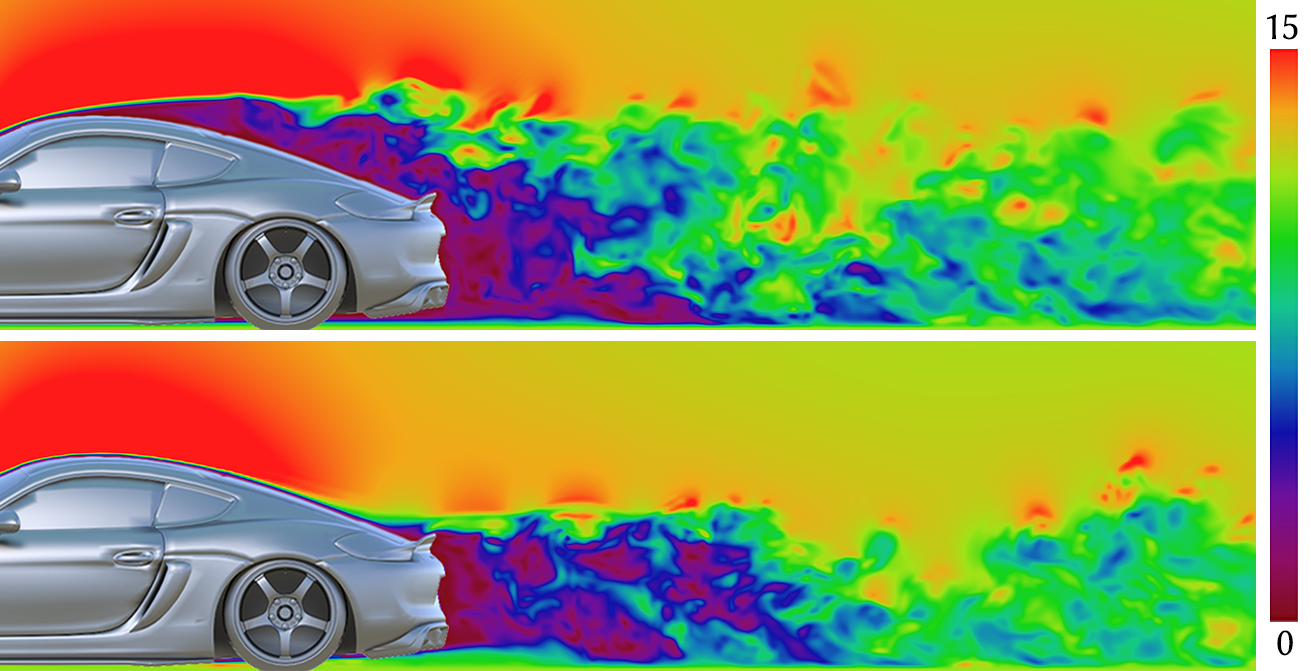
\includegraphics[width=0.95\columnwidth]{figures/comparsion_car_ib_ours.png}
  \bicaption[DI-IBM~\citep{Li-2020} (顶图) 与我们的图形方法 (底图) 进行气动仿真的对比]{DI-IBM~\citep{Li-2020} (顶图) 与我们的图形方法 (底图) 进行气动仿真的对比。速度场截面使用颜色可视化 (单位为$km/h$)。我们的仿真更贴近图~\ref{img:car_wind_tunnel} 中风洞的实际实验,而DI-IBM在车顶即开始发生边界层分离,不切合实际情况。}{Comparison of aerodynamic simulations. DI-IB method~\citepen{Li-2020} (top) vs. our result (bottom), using a visualization showing the color-coded velocity field magnitude (in $km/h$) of a cross section. While our simulation matches the wind-tunnel visualization of air flow around a car as Fig.~\ref{img:car_wind_tunnel} demonstrates, the DI-IB method, on the other hand, fails to have accurate boundary treatment, leading to unreasonable boundary layer separation at the top of the car.}
  \label{img:comparsion_car_ib_ours}
\end{figure}

\begin{figure}[!tb]
  \centering
    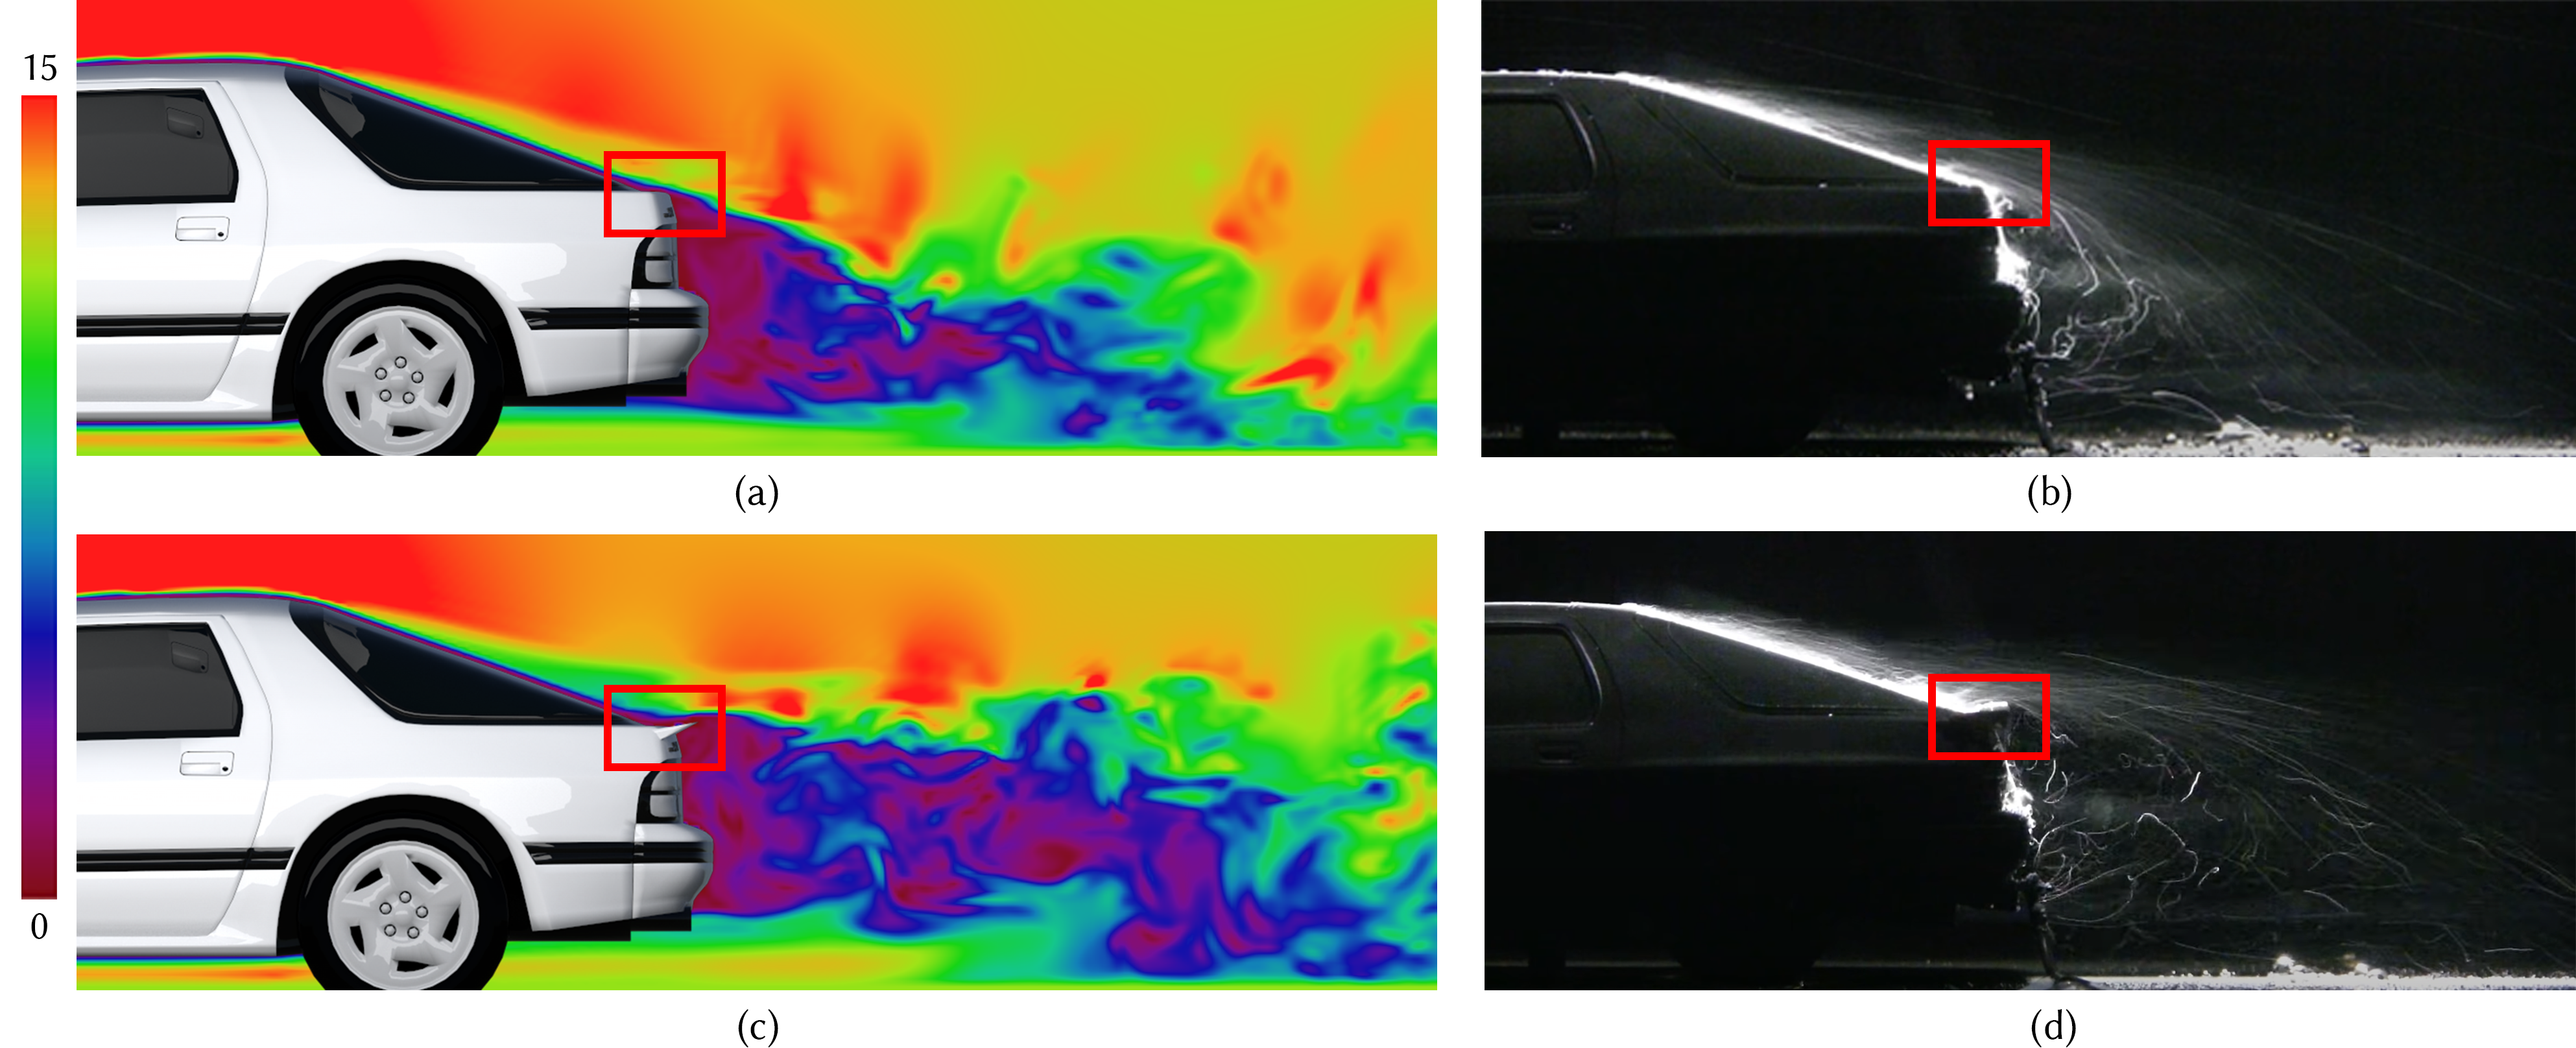
\includegraphics[width=0.99\columnwidth]{figures/comparsion_car_design.png}
  \bicaption[汽车的空气动力学设计]{汽车的空气动力学设计。通过我们的方法对没有尾翼的汽车进行仿真 (a),其结果与一个相似的车辆模型在风洞可视化的结果匹配 (b)。之后添加一个小型的扰流板 (图中红色方框) 到汽车尾部之后,仿真中的尾流发生显著变化 (c),与带有扰流板的风洞测试相似 (d)。这展示出我们的方法可以快速、有效地为气动外形设计服务。图中的速度模值单位为$km/h$。图 (b) 与 (d) 的版权来自~\citet{youtube_2014}。}{Aerodynamic design of a car model. Simulating the airflow around a car model without a spoiler using our solver (a) matches the wind tunnel visualization for a similar car model (b); A small and thin spoiler (in red box) added on the back of the car model (c) changes the wake flow of the car model in our simulation quite significantly, in line with a wind-tunnel test of a car model with a spoiler (d) --- indicating that our solver offers an efficient, yet predictive tool of air flows for computational shape design. The velocity magnitude is measured in $km/h$. Image (b) and (d) courtesy of~\citeten{youtube_2014}.}
  \label{img:comparsion_car_design}
\end{figure}

另外,DI-IBM有精度不足的问题,使得在湍流仿真时得不到正确结果,尤其是在固体边界层上。我们对一个向前运动的汽车模型进行气流仿真来说明这一问题,见图~\ref{img:comparsion_car_ib_ours}。对于汽车外形来说,气流的分离点一般位于汽车尾部,并且可以通过扰流板等进一步影响尾流走向 (如图~\ref{img:comparsion_car_design} (d) 中的风洞实验)。但仿真结果显示,DI-IBM预测的边界分离点在车顶,完全不符合实际风洞实验,而我们的方法可以正确预测边界的分离点 (两次仿真除边界处理外使用同样的参数设置)。

为了展示如扰流板这样的小且薄的结构对汽车周围流场的影响,我们还在图~\ref{img:comparsion_car_design} 中展示了有扰流板与无扰流板时汽车流场的仿真结果。从结果中我们可以看到,在添加了扰流板后,汽车的尾流发生了明显的变化。扰流板破坏了车身尾部表面的气流,在产生湍流的同时减少了车辆尾部的升力,从而提升了车辆在高速时的操控性。这两个例子展示出了我们的方法针对于计算机图形学中已有LBM方法的优势。

\begin{figure}[!tb]
  \centering
    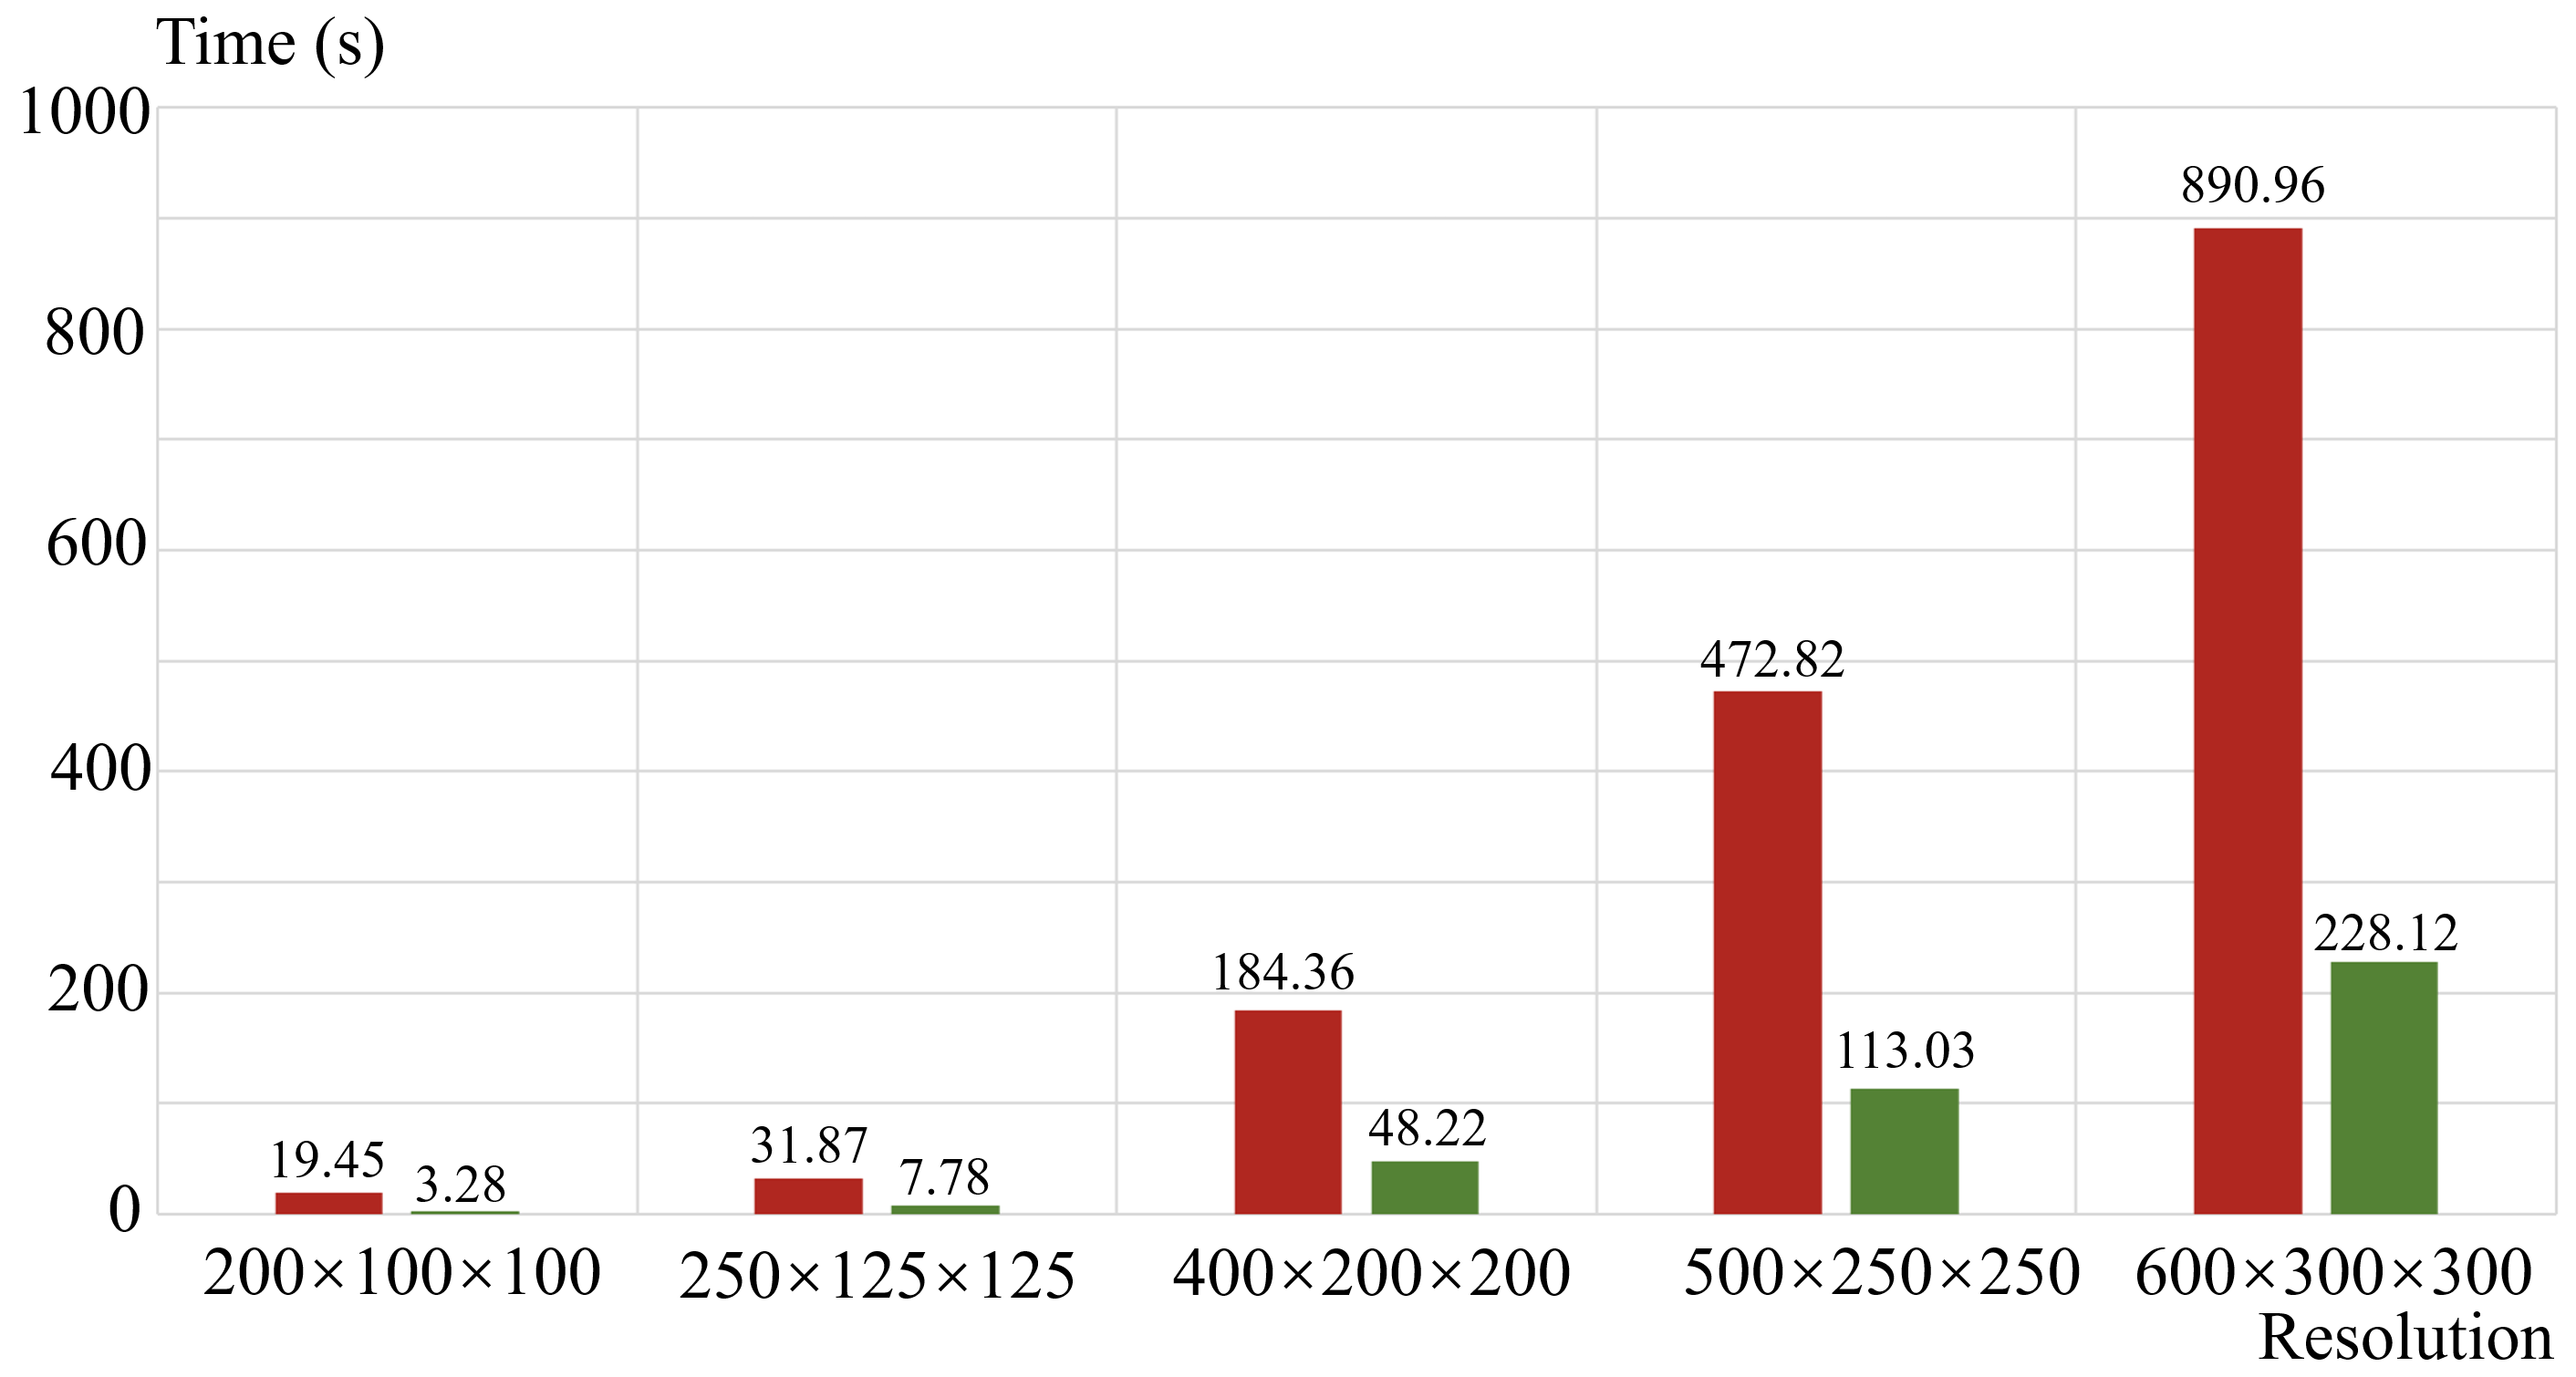
\includegraphics[width=0.93\columnwidth]{figures/performance.png}
  \bicaption[性能对比]{性能对比。我们将我们的方法 (绿色) 与~\citep{Li-2020,Chen-2021} 中的动理学求解方法 (红色) 进行比较,比较用例为图~\ref{img:comparsion_car_ib_ours} 中所示的汽车仿真,仿真时长为1秒。在同一张NVIDIA RTX 3090 GPU上得到的测试结果显示我们的方法在所有分辨率上都有显著的性能提升。}{Performance comparison. We compare the efficiency of the kinetic solver from~\citepen{Li-2020,Chen-2021} (red) with our kinetic solver (green) based on one second of simulation of the car model shown in Fig.~\ref{img:comparsion_car_ib_ours} and both executed on a same NVIDIA RTX 3090 GPU, showing significant performance improvement for all grid resolutions.}
  \label{img:Performance}
\end{figure}

\paragraph{性能对比}
在~\citep{Li-2020} 与~\citep{Chen-2021} 中,作者已经通过对比,说明了动理学方法的计算效率是显著优于N-S方法的。这种优势在湍流流固耦合仿真中更加明显,因为需要的时间步长更小。由于我们的方法与这些工作的框架相同,结合上述的各项优化,使得我们的方法在性能上更有优势。我们在同一张NVIDIA RTX 3090 GPU上,进行了多个分辨率的对比,结果显示我们的方法在所有的分辨率上都有显著提升 (见图~\ref{img:Performance})。通过代码性能分析,我们分析出两个使性能得以提升的主要因素:第一个是基于LU分解的碰撞运算符简化~\citep{fei2018three} 显著提升了GPU占用率,第二个是使用了几何近似优化之后,我们的混合边界处理比起之前工作使用的DI-IBM,计算量要更小。这两点使得我们的GPU计算效率得以提升。

\section{方法的局限性}
虽然我们的方法展示出了优秀的通用性与数值结果,我们的方法依旧有一定的局限性。
首先,由于我们使用了基于采样点的几何计算近似,当固体包含尖角的时候,是否需要应用反弹边界可能发生误判。增加采样点数量或使用自适应采样可以提升精度,但是也会同时提升显存需求。第二,对固体所受的力和力矩的计算也受制于对固体外形的近似。如我们的亚网格近似无法真实反应物体的几何形状,会影响固体受力计算的精度。最后,我们的方法没有讨论对可变形物体的支持。对于可变形的物体,我们的方法需求一个更高效的采样方法,以每帧更新物体表面的采样点。这有待后续研究。

我们也要指出,我们通过定性地复现物理现象,与图形学中现有的方法进行了比较,并证明了我们的仿真方法的精度。但我们并无法使用该方法定量地进行物理量计算,或应用于对精度较为敏感的应用场景。我们在第~\ref{chap:sig23} 章中提出一系列新的方法以解决这一问题。

\section{总结}
在本章中,我们提出了一个基于动理学方法的混合边界处理方法,以处理在流固双向耦合。我们的方法可以有效、统一地同时处理厚、薄物体,并可以稳定、快速地完成仿真,得到视觉上可信的结果。我们的方法充分利用了反弹边界与尖锐界面浸没边界法优点的互补性,包含双面反弹边界处理与单边的速度修正,与双向耦合所需的固体受力计算。
我们基于边界采样点提出了高效的几何近似算法与对应的GPU并行实现,以提升整体计算效率。我们的方法在效率与精度上都超越了现有的计算机图形学中的LBM算法,并在强湍流中依然可以捕捉到正确的物理现象。

基于我们方法高效、灵活的特点,我们的方法十分适用于图形学中的视觉动画制作。虽然我们展示了一些定性的物理现象复现,但是我们需要指出,若要定量地进行物理量计算,需要使用非常高的分辨率进行仿真。这势必会带来很大的内存 (及显存) 消耗。为了减轻这一问题,我们在下一章中提出高精度的多分辨率流体仿真方法,讨论面向更高精度需求应用的流体仿真框架。
% 我们展示了我们的方法与其它方法和实际实验的对比,和一系列的仿真结果,包括不同的几何形状在流体中的单向或双向耦合仿真,及我们的方法在快速交互式设计中的应用。